%%*************************************************************************
%% Legal Notice:
%% This code is offered as-is without any warranty either expressed or
%% implied; without even the implied warranty of MERCHANTABILITY or
%% FITNESS FOR A PARTICULAR PURPOSE! 
%% User assumes all risk.
%% In no event shall IEEE or any contributor to this code be liable for
%% any damages or losses, including, but not limited to, incidental,
%% consequential, or any other damages, resulting from the use or misuse
%% of any information contained here.
%%
%% All comments are the opinions of their respective authors and are not
%% necessarily endorsed by the IEEE.
%%
%% This work is distributed under the LaTeX Project Public License (LPPL)
%% ( http://www.latex-project.org/ ) version 1.3, and may be freely used,
%% distributed and modified. A copy of the LPPL, version 1.3, is included
%% in the base LaTeX documentation of all distributions of LaTeX released
%% 2003/12/01 or later.
%% Retain all contribution notices and credits.
%% ** Modified files should be clearly indicated as such, including  **
%% ** renaming them and changing author support contact information. **
%%
%% File list of work: IEEEtran.cls, IEEEtran_HOWTO.pdf, bare_adv.tex,
%%                    bare_conf.tex, bare_jrnl.tex, bare_jrnl_compsoc.tex
%%*************************************************************************

% Note that the a4paper option is mainly intended so that authors in
% countries using A4 can easily print to A4 and see how their papers will
% look in print - the typesetting of the document will not typically be
% affected with changes in paper size (but the bottom and side margins will).
% Use the testflow package mentioned above to verify correct handling of
% both paper sizes by the user's LaTeX system.
%
% Also note that the "draftcls" or "draftclsnofoot", not "draft", option
% should be used if it is desired that the figures are to be displayed in
% draft mode.
%
\documentclass[journal]{IEEEtran}

\usepackage{cite}
%
\ifCLASSINFOpdf
  \usepackage[pdftex]{graphicx}
\else
\fi
\usepackage[cmex10]{amsmath}
\usepackage[tight,footnotesize]{subfigure}

% *** Do not adjust lengths that control margins, column widths, etc. ***
% *** Do not use packages that alter fonts (such as pslatex).         ***
% There should be no need to do such things with IEEEtran.cls V1.6 and later.
% (Unless specifically asked to do so by the journal or conference you plan
% to submit to, of course. )


% correct bad hyphenation here
\hyphenation{op-tical net-works semi-conduc-tor}

\newcommand{\ETslash}{\ensuremath{E_{\mathrm{T}}\hspace{-1.1em}/\kern0.45em}}


\begin{document}
\title{CMS ECAL calibration and timing: \\ performance during LHC Run I and future prospects}

\author{Emanuele~Di~Marco~on~behalf~of~the~CMS~Collaboration,~\IEEEmembership{CERN, CH-1211 Geneva 23, Switzerland}}

\maketitle


\begin{abstract}
%\boldmath
The CMS ECAL is a high-resolution, hermetic, and homogeneous electromagnetic calorimeter made of 75,848 scintillating lead tungstate crystals. It relies on precision calibration of energy and timing in order to achieve and maintain its design performance. A set of inter-calibration procedures is carried out to normalize the differences in crystal light yield and photo-detector response between channels. Different physics channels such as low mass di-photon resonances, electrons from W and Z decays and the azimuthal symmetry of low energy deposits from minimum bias events are used. A laser monitoring system is used to measure and correct for response changes, which arise mainly from the harsh radiation environment at the LHC. The energy reconstruction algorithms and its calibration techniques are discussed along with the performance evolution during Run I and prospects for Run II. Moreover, the ECAL can be used to accurately determine the time of flight of photons. The stability of the time measurement required to maintain the energy resolution is on the order of 1 ns. Conclusions are drawn for the performance to be expected from 2015 onwards, following the start of the LHC Run II.
\end{abstract}

% Note that keywords are not normally used for peerreview papers.
\begin{IEEEkeywords}
\end{IEEEkeywords}

\IEEEpeerreviewmaketitle



\section{Introduction}
\label{sec:introduction}
\IEEEPARstart{T}{he} Compact Muon Solenoid (CMS) experiment \cite{Chatrchyan:2008aa} is a general purpose experiment at the Large Hadron Collider (LHC) at CERN, designed to search for the standard model (SM) Higgs boson and for new physics beyond the SM. Many of these searches involve electrons or photons in the final state, and the electromagnetic calorimeter (ECAL) plays an essential role in their reconstruction and identification.

The CMS ECAL \cite{CMS:1997ema} has been designed to achieve an excellent energy resolution and energy scale linearity, which are key points of the searches of the Higgs boson in final states involving electromagnetic particles and in particular in the H$\to\gamma\gamma$ \cite{Khachatryan:2014ira} and H$\to Z^{(\ast)}Z^{(\ast)}\to 4\ell$ channels \cite{Chatrchyan:2013mxa}, and to guarantee a good hermeticity, allowing good performances on the measurement of the missing transverse energy ($\ETslash$).

It is a homogeneous and hermetic calorimeter containing 61200 lead tungstate ($\rm PbWO_4$) scintillating crystals mounted in the barrel (EB), closed at each end by endcaps (EE) each containing 7324 crystals. The choice of the $\rm PbWO_4$ with a radiation length $X_0=0.85$ cm and a Moliere radius $R_0$=2.19 cm ensures the compactness of the detector and the radiation hardness necessary to cope with the harsh environment of the collisions at LHC. The scintillation light is read by avalanche photodiodes (APDs) and vacuum phototriodes (VPTs) in the EB and EE
respectively, resulting in an average of 4.5 photoelectrons per MeV deposited in the crystals. 

In the EB, which covers the region $\vert\eta\vert<$1.48, the crystals have a truncated pyramidal shape (2.2$\times$2.2 cm$^2$ on the frontal face, and a length of 23 cm) and they are organized in 36 supermodules, 18 on each side of the beam interaction point, each with 20 channels along $\phi$ and 85 along $\eta$, divided in four modules along $\eta$. The EE extends the coverage to $\vert\eta\vert$=3.0, with the crystals (2.86$\times$2.86 cm$^2$ on the frontal face, and a length of 22 cm) arranged in an x-y grid. A preshower detector (ES), based on lead absorbers equipped with silicon strip sensors, is installed in front of EE covering a fiducial region $1.65<\vert\eta\vert<2.6$.

The ECAL is installed inside the CMS superconductive coil and operate in the strong magnetic field of 3.8 T, used to reconstruct the momentum of charged particle in the CMS silicon tracker which covers the region up to $\vert\eta\vert=2.5$.



\section{Energy reconstruction}
\label{sec:energyreco}
\IEEEPARstart{T}{he} electrical signal from the photo-detectors, after amplification and shaping by a multi-gain preamplifier (MGPA) is digitized by ADCs at a frequency of 40 MHz. An amplification with three possible gains and a further logic chooses the highest non-saturated digital value, allowing a dynamic range of about $5 \times 10^4$ from the least significant bit of about 35 MeV to saturation at 1.7 TeV in the barrel. The data read out consists of a series of consecutive digitizations, corresponding to a sequence of samplings of the signal at 40 MHz. A set of 10 consecutive samplings is readout, and the signal amplitude is reconstructed using these samplings. 

During the LHC Run I a digital filtering algorithm was used, where the signal amplitude is estimated as the linear combination of the $N=10$ samples $S_i$:
%
\begin{equation}
\hat{\cal A}=\sum_{i=1}^{N} w_i \times S_i
\end{equation}
%
where the weights $w_i$ were calculated by minimizing the variance of $\hat{\cal A}$. For a detailed description of this method the reader is referred to \cite{Bruneliere:2006ra}. This method is fast enough to be run offline and online in the High Level Trigger (HLT), and provides an optimal filter of the electronics noise. This is estimated event-by-event by the average of the first three digitized pedestal-only samples.

For LHC Run II the center of mass energy will be higher ($\sqrt{s}=$13 TeV), and the instantaneous luminosity is expected to increase by a factor two. The average number of pile-up interactions per bunch crossing (BX) is going to be higher, within the range [20--40]. Finally, the bunch spacing will be 25 ns, with respect the 50 ns one used during LHC Run I. The reduced bunch spacing increases the contribution of out-of-time (other bunch crossing) interactions to the energy estimate. Several methods have been investigated to mitigate the effect of pile-up, while keeping the noise filtering optimal. The method that have been investigated are: a single sample on the signal pulse maximum, a Z-transform converting the discrete time signal into the frequency domain~\cite{Gadomski:1992xu}, and a template fit with multiple components (``multi-fit''). The last one is the algorithm under characterization with large simulation samples for Run II and it is described here.
The multi-fit algorithm estimates the in-time signal amplitude and up to 9 out of time amplitudes by minimization of the $\chi^2$, given by:
\begin{equation}
\label{eqn:chi2multifit}
\chi^2 = \sum_{i=1}^{N} \frac{\left(\sum_{j=1}^M {\cal A}_{j}p_{ij} - S_i \right)^2}{\sigma^2_{S_i}}
\end{equation}
where ${\cal A}_{j}$ are the amplitudes of up to $M=10$ interactions. The pulse templates $\mathbf{\vec p}_j$ for each bunch crossing $j$ have the same shape, but a time shift of 25 ns for each BX hypothesis. The amplitudes for the BXs from -5 to -1 (early out-of-time pile-up), 0 (sum of the in-time pulse and in-time pile-up pulses), and +1 to +4 (late out-of-time pile-up) are floated in the fit.
The pulse templates for each crystal are measured from low pile-up $pp$ collision data recorded by CMS at the beginning of 2013. Examples of the pulse shape templates measured for some crystals in the barrel are shown in Fig.~\ref{fig:pulse_shapes_template}. They are compared with the simulation, which is generated from the pulse shape measured in test beam data, with its envelope band, represented by time jitter variations and the fluctuations in the arrival time of the photons to the ECAL.

The sample-to-sample correlations in the pulse templates are taken into account by a $N \times N$ covariance matrix ($\sigma_{p_i}$) measured from the same data. The total electronic noise and its covariance matrix $\sigma_{S_i}$ are estimated by using local runs taken during no-beams periods, with a frequency of about one week, and stored into the conditions database. The correlation of the noise among the time samples decreases when increasing the interval among them, with an exponential constant which is characteristic of the shaping time of the electronics, reaching a plateau dominated by the low-frequency pickup noise. This matrix is very stable within the different barrel or endcap partitions, as shown by the autocorrelation function (top row of the normalized covariance matrix) in Fig.~\ref{fig:noise_autocorrelation}. The total noise is taken as the quadrature sum of the pulse shapes uncertainty and the electronic noise: $\sigma_{S_i}^2+\sum_{j=1}^M {\cal A}_{j}\sigma_{p_ij}^2$. The former dominates the uncertainty of low energy pulses, while the latter dominate the high energy pulses.
%
\begin{figure}[!t]
  \begin{center}
    \subfigure[]{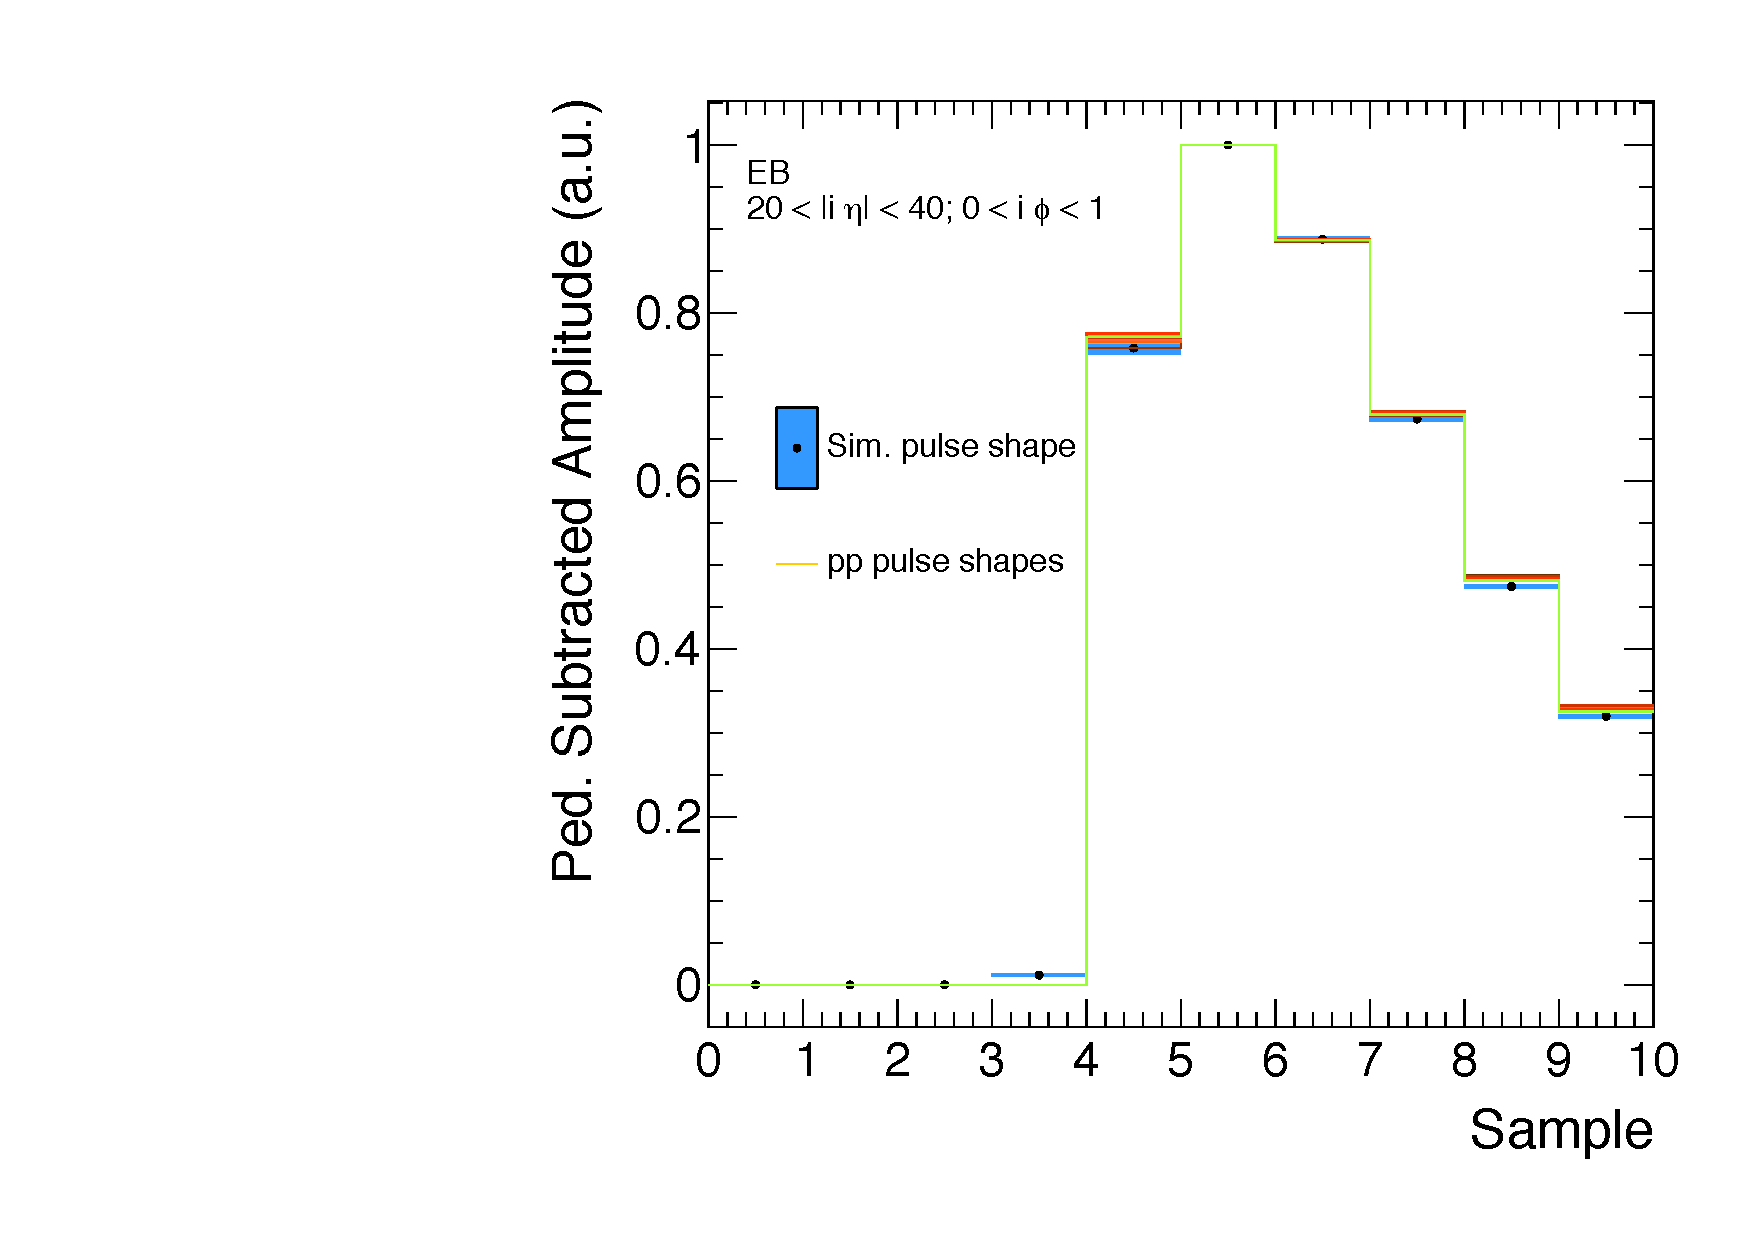
\includegraphics[width=3.0in]{template_EB}\label{fig:pulse_shapes_template}}
    \subfigure[]{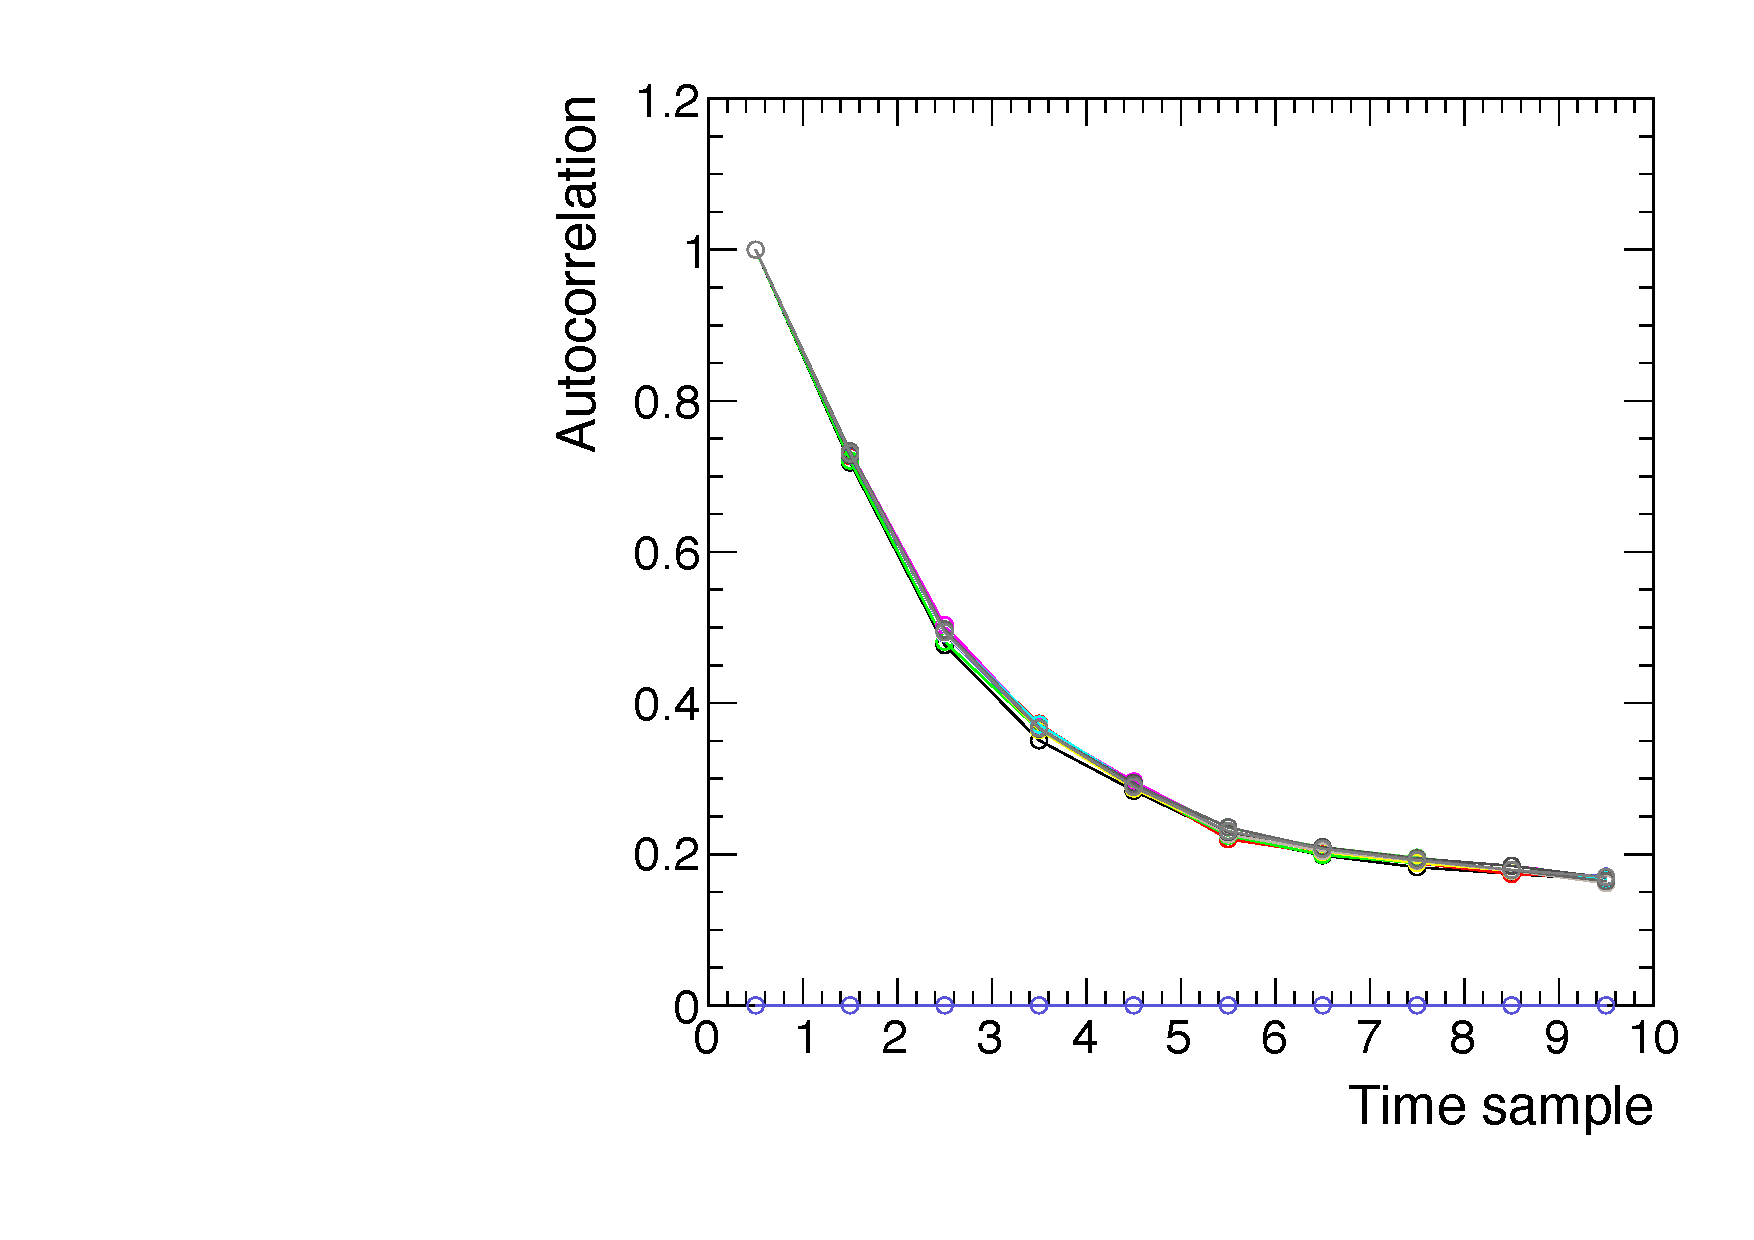
\includegraphics[width=3.0in]{autocorrelation_barrel}\label{fig:noise_autocorrelation}}
    \caption{Examples of pulse shapes measured on data in the barrel, after time inter-calibration, compared with the one used in the simulation, averaged over the full barrel, with its uncertainty band (a). Example of the noise autocorrelation measured on 2012 data, for several partitions of the barrel (b). \label{fig:pulse_shapes} }
  \end{center}
\end{figure}


Given the number of allowed pulses is $N=10$ for the 25 ns bunch spacing case, in order to have always a constrained fit with the 10 digitized samples we impose that each of the amplitudes is positive. The technique of Non-Negative-Least-Squares \cite{nnls} is adopted to perform the $\chi^2$ minimization of Eq.~\ref{eqn:chi2multifit} with such a constraint, within $\approx$ 10 ms/event with an average number of pile-up interaction of 40 and 25 ns bunch spacing. Having such a fast algorithm is necessary especially for the HLT needs. Examples of one fit for a hit in the barrel and a hit in the endcap are shown in Fig.~\ref{fig:multifits}.
%
\begin{figure}[!t]
  \begin{center}
    \subfigure[]{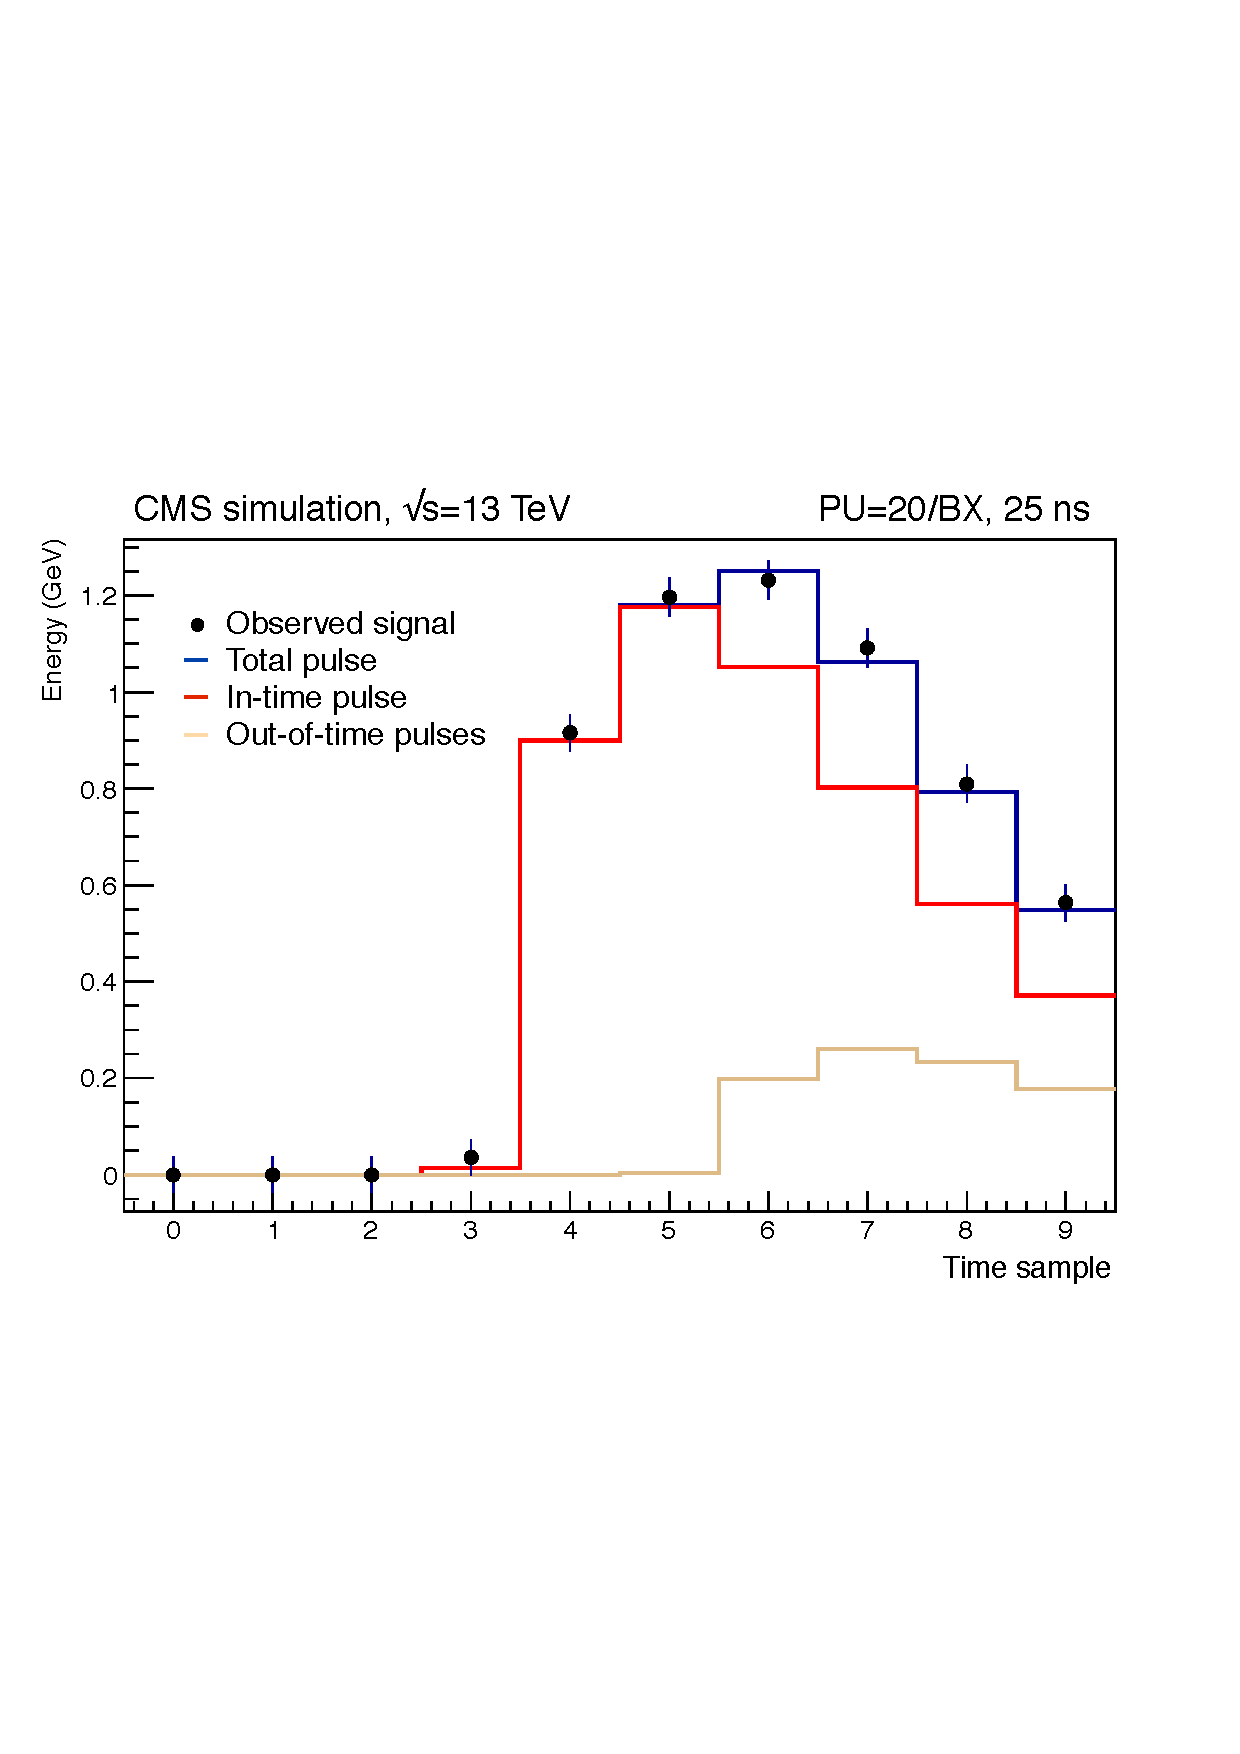
\includegraphics[width=3.1in]{multifit_EB}\label{fig:multifit_EB}}
    \subfigure[]{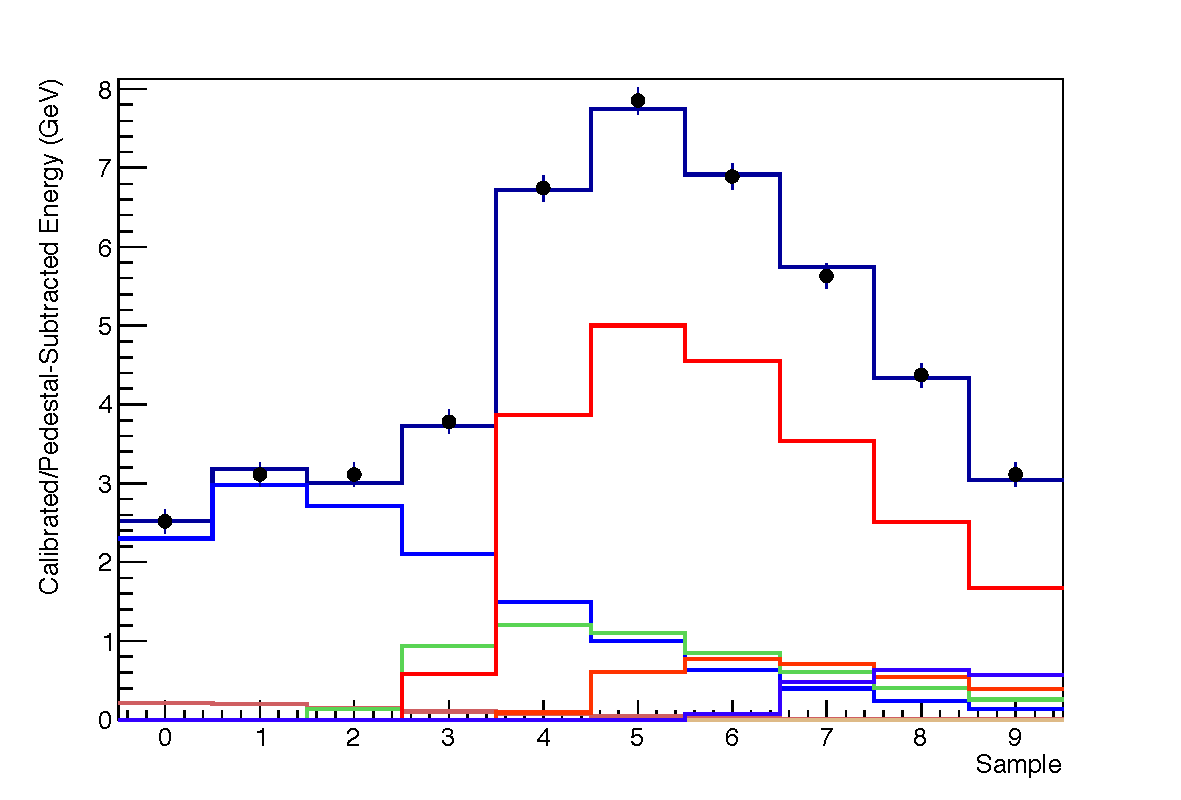
\includegraphics[width=3.1in]{multifit_EE}\label{fig:multifit_EE}}
    \caption{Example of fitted pulses in simulated events with 20 average pile-up events and 25 ns bunch spacing. Dots represent the 10 digitized samples, red distribution (other light colors) represent the fitted in-time (out-of time) pulses with positive amplitude. Dark blue histogram represents the sum of all the fitted contributions. A barrel hit (a) and a endcap hit (b).  \label{fig:multifits} }
  \end{center}
\end{figure}


With simulated unconverted photon gun samples (no material in front of ECAL) the impact of the residual contribution of the out-of-time pile-up to the energy resolution is expected to be suppressed to a negligible level in both the barrel and in the endcap. The improvement with respect the Run I reconstruction algorithm for the 25 ns bunch spacing conditions is substantial especially for low $p_T$ photons and electrons, given the relatively higher pile-up contribution to the energy, and it is still significant for high $p_T$ ones ($p_T>$50 GeV). The new local reconstruction is thus expected to reduce the pile-up dependency in the electromagnetic components of reconstructed jets and $\ETslash$ to a small level with 25 ns bunch spacing and high number of pile-up interactions.

Electrons and photons deposit their energy over many ECAL channels, in fact the electromagnetic shower is not completely contained in a single crystal and, more importantly, the presence of material in front of ECAL causes conversion of photons and bremsstrahlung from electrons, and the radiated energy is spread along $\phi$ by the strong magnetic field. Clustering algorithms are used to collect the energy deposits in ECAL, including the ones related to the radiated energy. For the LHC Run II the clustering algorithms will be changed such that also the correlation in the $\eta-\phi$ plane of the radiated energy due to the combined effect of the magnetic field and material budget distribution is taken into account in a ``banana-like'' shape. The electron or photon energy is then estimated as:
\begin{equation}
\label{eqn:energy}
E_{e,\gamma} = F_{e,\gamma}\left[G \times \sum_i(C_i \times S_i(t) \times {\cal A}_i + E_{ES}\right]
\end{equation}
where the sum is performed over all the clustered channels. The amplitude measured in the $i$-th channel is labeled by ${\cal A}_i$, while $S_i(t)$ is a time dependent correction that account for time variation of the channel response mainly due to changes in the crystal transparency, $C_i$ is a relative calibration constant which takes into account differences in the crystal light yields and photo-detector responses and $G$ is a scale factor converting the digital scale into GeV. For clusters in the endcap region the corresponding energy in the preshower ($E_{ES}$) is added. Finally $F_{e,\gamma}$ is particle dependent correction applied to the clustered energy. It accounts for effects affecting the energy reconstruction related to the geometry of the detector, the upstream material, and the clustering of energy emitted by bremsstrahlung or photon conversion. The pile-up dependency of the energy scale and its correlation with the cluster shape and position is taken into account by a multivariate algorithm trained on simulated samples of electrons and photons.  Residual data-simulation differences are accounted by in-situ measurements with copious physics processes producing electrons and photons in the final state.



\section{Energy calibrations}
\label{sec:energycalibration}
\IEEEPARstart{I}{n} the following the calibration of the ECAL response and the resulting performance in the data collected in the 2012 are illustrated. The procedures are expected to stay mostly untouched during the Run II, while reoptimizations of the calibration streams are necessary, to cope with the increased rate of non genuine electrons in jets and the larger data volume at HLT due to the higher occupancy of in-time and out-of-time pile-up particles. For a detailed description of the ECAL calibration procedures the reader is referred to~\cite{Chatrchyan:2013dga}.

\subsection{Corrections for the change of the response in time}
Radiation can create color centers in the crystals reducing their transparency and therefore reducing the measured response to the deposited energy. The color centers partially anneal with thermal energy so that the loss in transparency depends on the dose rate, which for ECAL varies along $\eta$, and in absence of radiation a partial recovery of the transparency is observed.
Despite the good radiation resistance of the $PbWO_4$ crystals, a residual radiation damage remains and needs to be corrected for. Thus, the changes in transparency are measured by a dedicated ``laser monitoring'' system \cite{Anfreville:2007zz} (LM) which injects a laser light ($\lambda=440$ nm, close to the peak of the scintillation light spectrum for $PbWO_4$) into each single crystal, with a cycle of 40 minutes. The change in transparency ($R/R_0$) does not directly measures the change in response for the scintillation light ($S/S_0$) since the two have different spectra and the optical photons travel different paths to reach the photo-detectors, but they can be related by a power law:
\begin{equation}
\frac{S}{S_0} = \left(\frac{R}{R_0}\right)^\alpha
\end{equation}

By the end of the LHC Run I in 2012 the loss in transparency was less than 6\% in EB and less than 30\% in the EE region within the tracker acceptance ($\vert\eta\vert<2.5$), while it reached 70\% in the most forward EE region. The corrections for transparency loss (LC) can be validated with collisions data, by looking at the stability of the reconstructed invariant mass of $\pi^0$ and of the distribution of $E/p$ for isolated electrons, where $E$ is the energy measured in the calorimeter and $p$ is the momentum measured in the tracker. Applying the LC the stability is better than 0.1\% in the barrel and 0.4\% in the endcaps.  Stability of the $E/p$ scale during 2012, before (red) and after (green) the LC, for the ECAL barrel are shown in Fig.~\ref{fig:EoP_2012}. The projections along the Y axis are shown in the histograms on the right side.
 The resulting residual imperfection of the LC due to the dispersion in the values of $\alpha$ can be recovered by allowing a time dependence of the calibrations constants as explained in the next section. 
%
\begin{figure}[!t]
  \begin{center}
    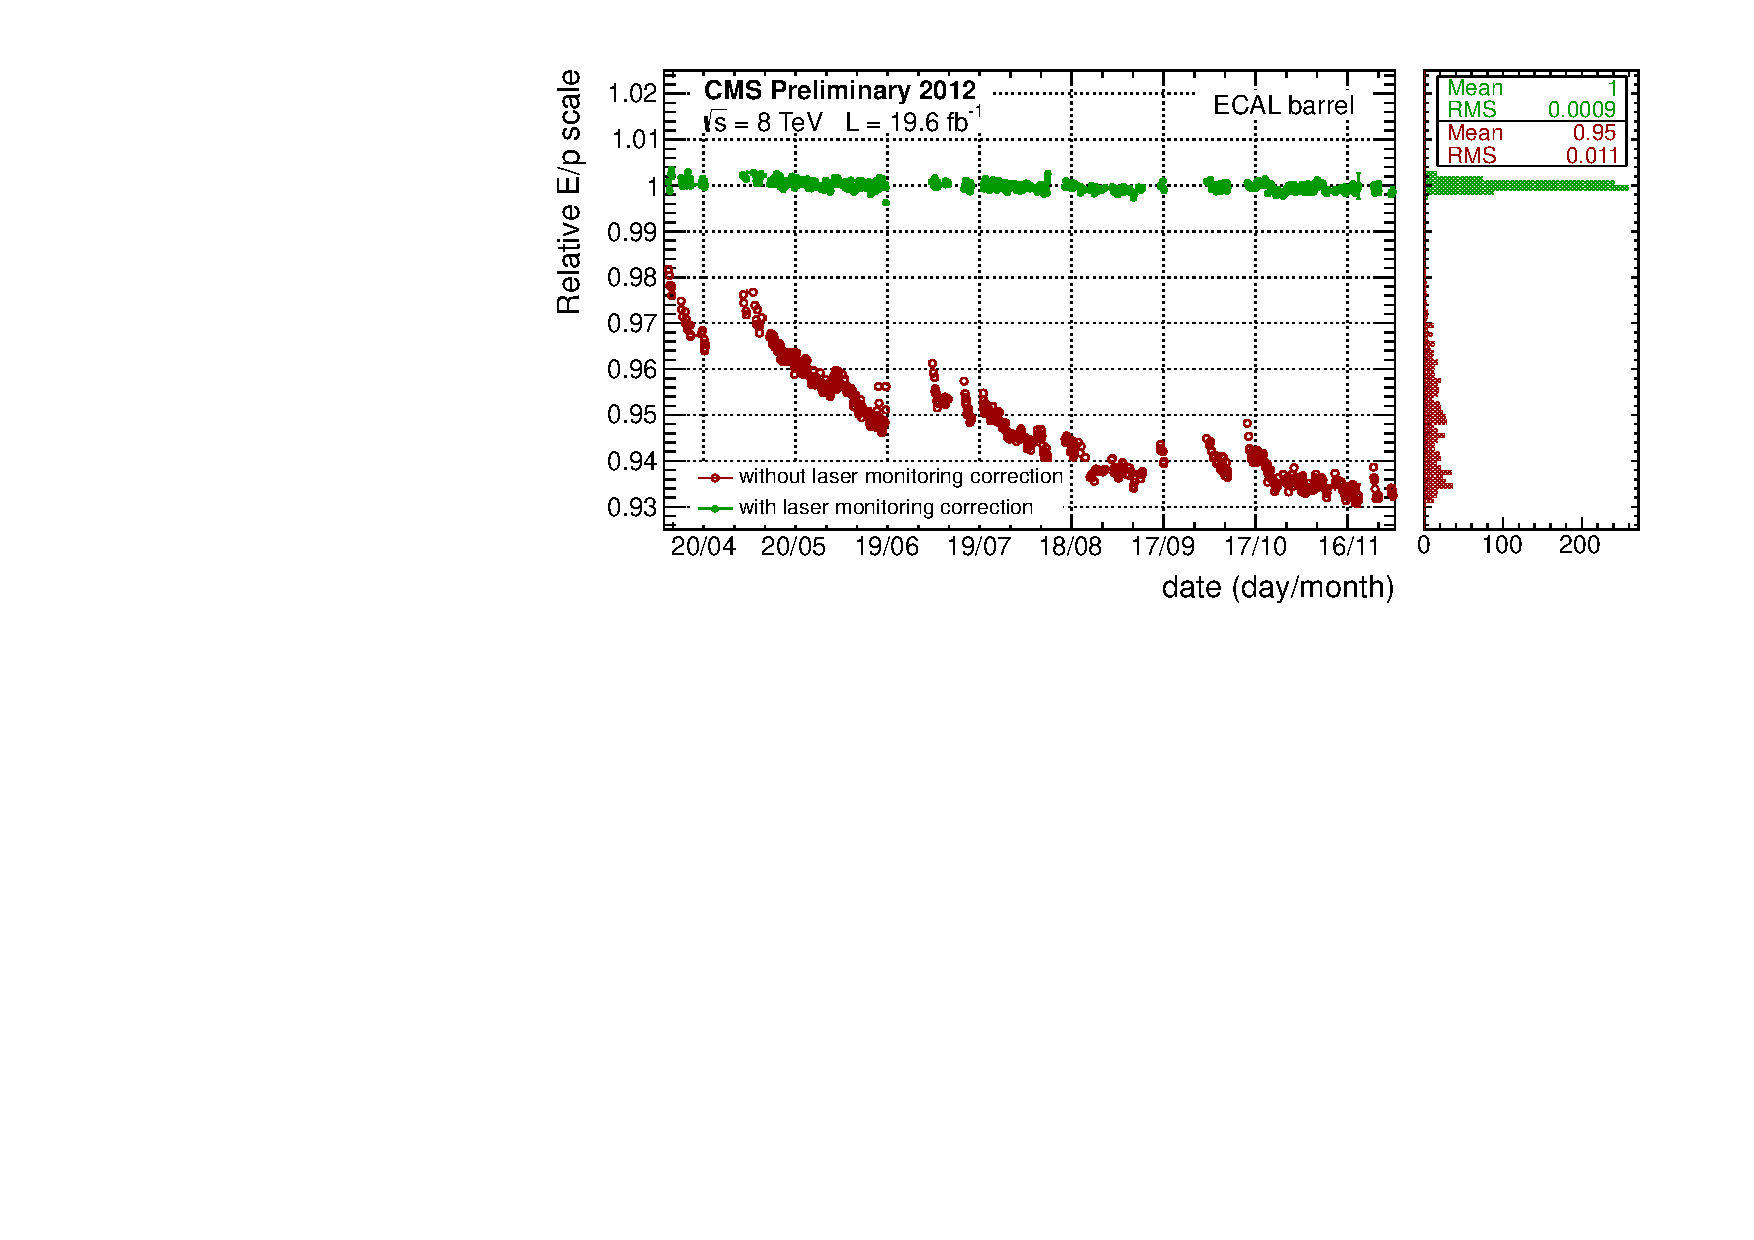
\includegraphics[width=3.5in]{EoP_EB_Winter2013}
    \caption{History plot for 2012 data of the ratio of electron energy E, measured in the ECAL Barrel, to the electron momentum p, measured in the tracker.  The electrons are selected from $W\to e\nu$ decays. Each point in the plot is computed from 20000 selected events with the reconstructed electron located in the ECAL Barrel. \label{fig:EoP_2012}}
  \end{center}
\end{figure}


For the Run II one of the main challenges is to preserve the number of the $W\to e\nu$ events, given that the physics single electron stream used in 2012 will be pre-scaled due to the higher electron misidentification probability with larger pile-up. A dedicated HLT stream has thus been developed that reduces the bandwith occupancy by trasmitting to disk only the hits of the tracker and ECAL partitions traversed by the reconstructed electron. In addition, several global event variables are saved in this stream to define the event selection and the cluster corrections, such as the $\ETslash$, the average density of the event, and the HCAL over ECAL cluster energy ($H/E$) ratio.  An event display of a $W\to e\nu$ event with the standard reconstruction and with the content stripping done for the HLT stream is shown in Fig.~\ref{fig:elestream}. The figure Fig.~\ref{fig:elestream_before} shows the $\ETslash$ when the full event content is available and the offline reconstruction is run. The $\slash E_T$ in the stripped event content would by construction be back-to-back to the electron transverse momentum, so the HLT $\ETslash$ is retained and used for the selection, as shown in Fig.~\ref{fig:elestream_after}. Since it is reconstructed by the HLT candidates, it provides only an approximation of the offline one, but it is sufficiently good to provide a hig offline/online efficiency ratio. Depending on the amount of information around the electron retained, the event size is reduced to 10\%--20\% of the original one.
%
\begin{figure}[!t]
  \begin{center}
    \subfigure[]{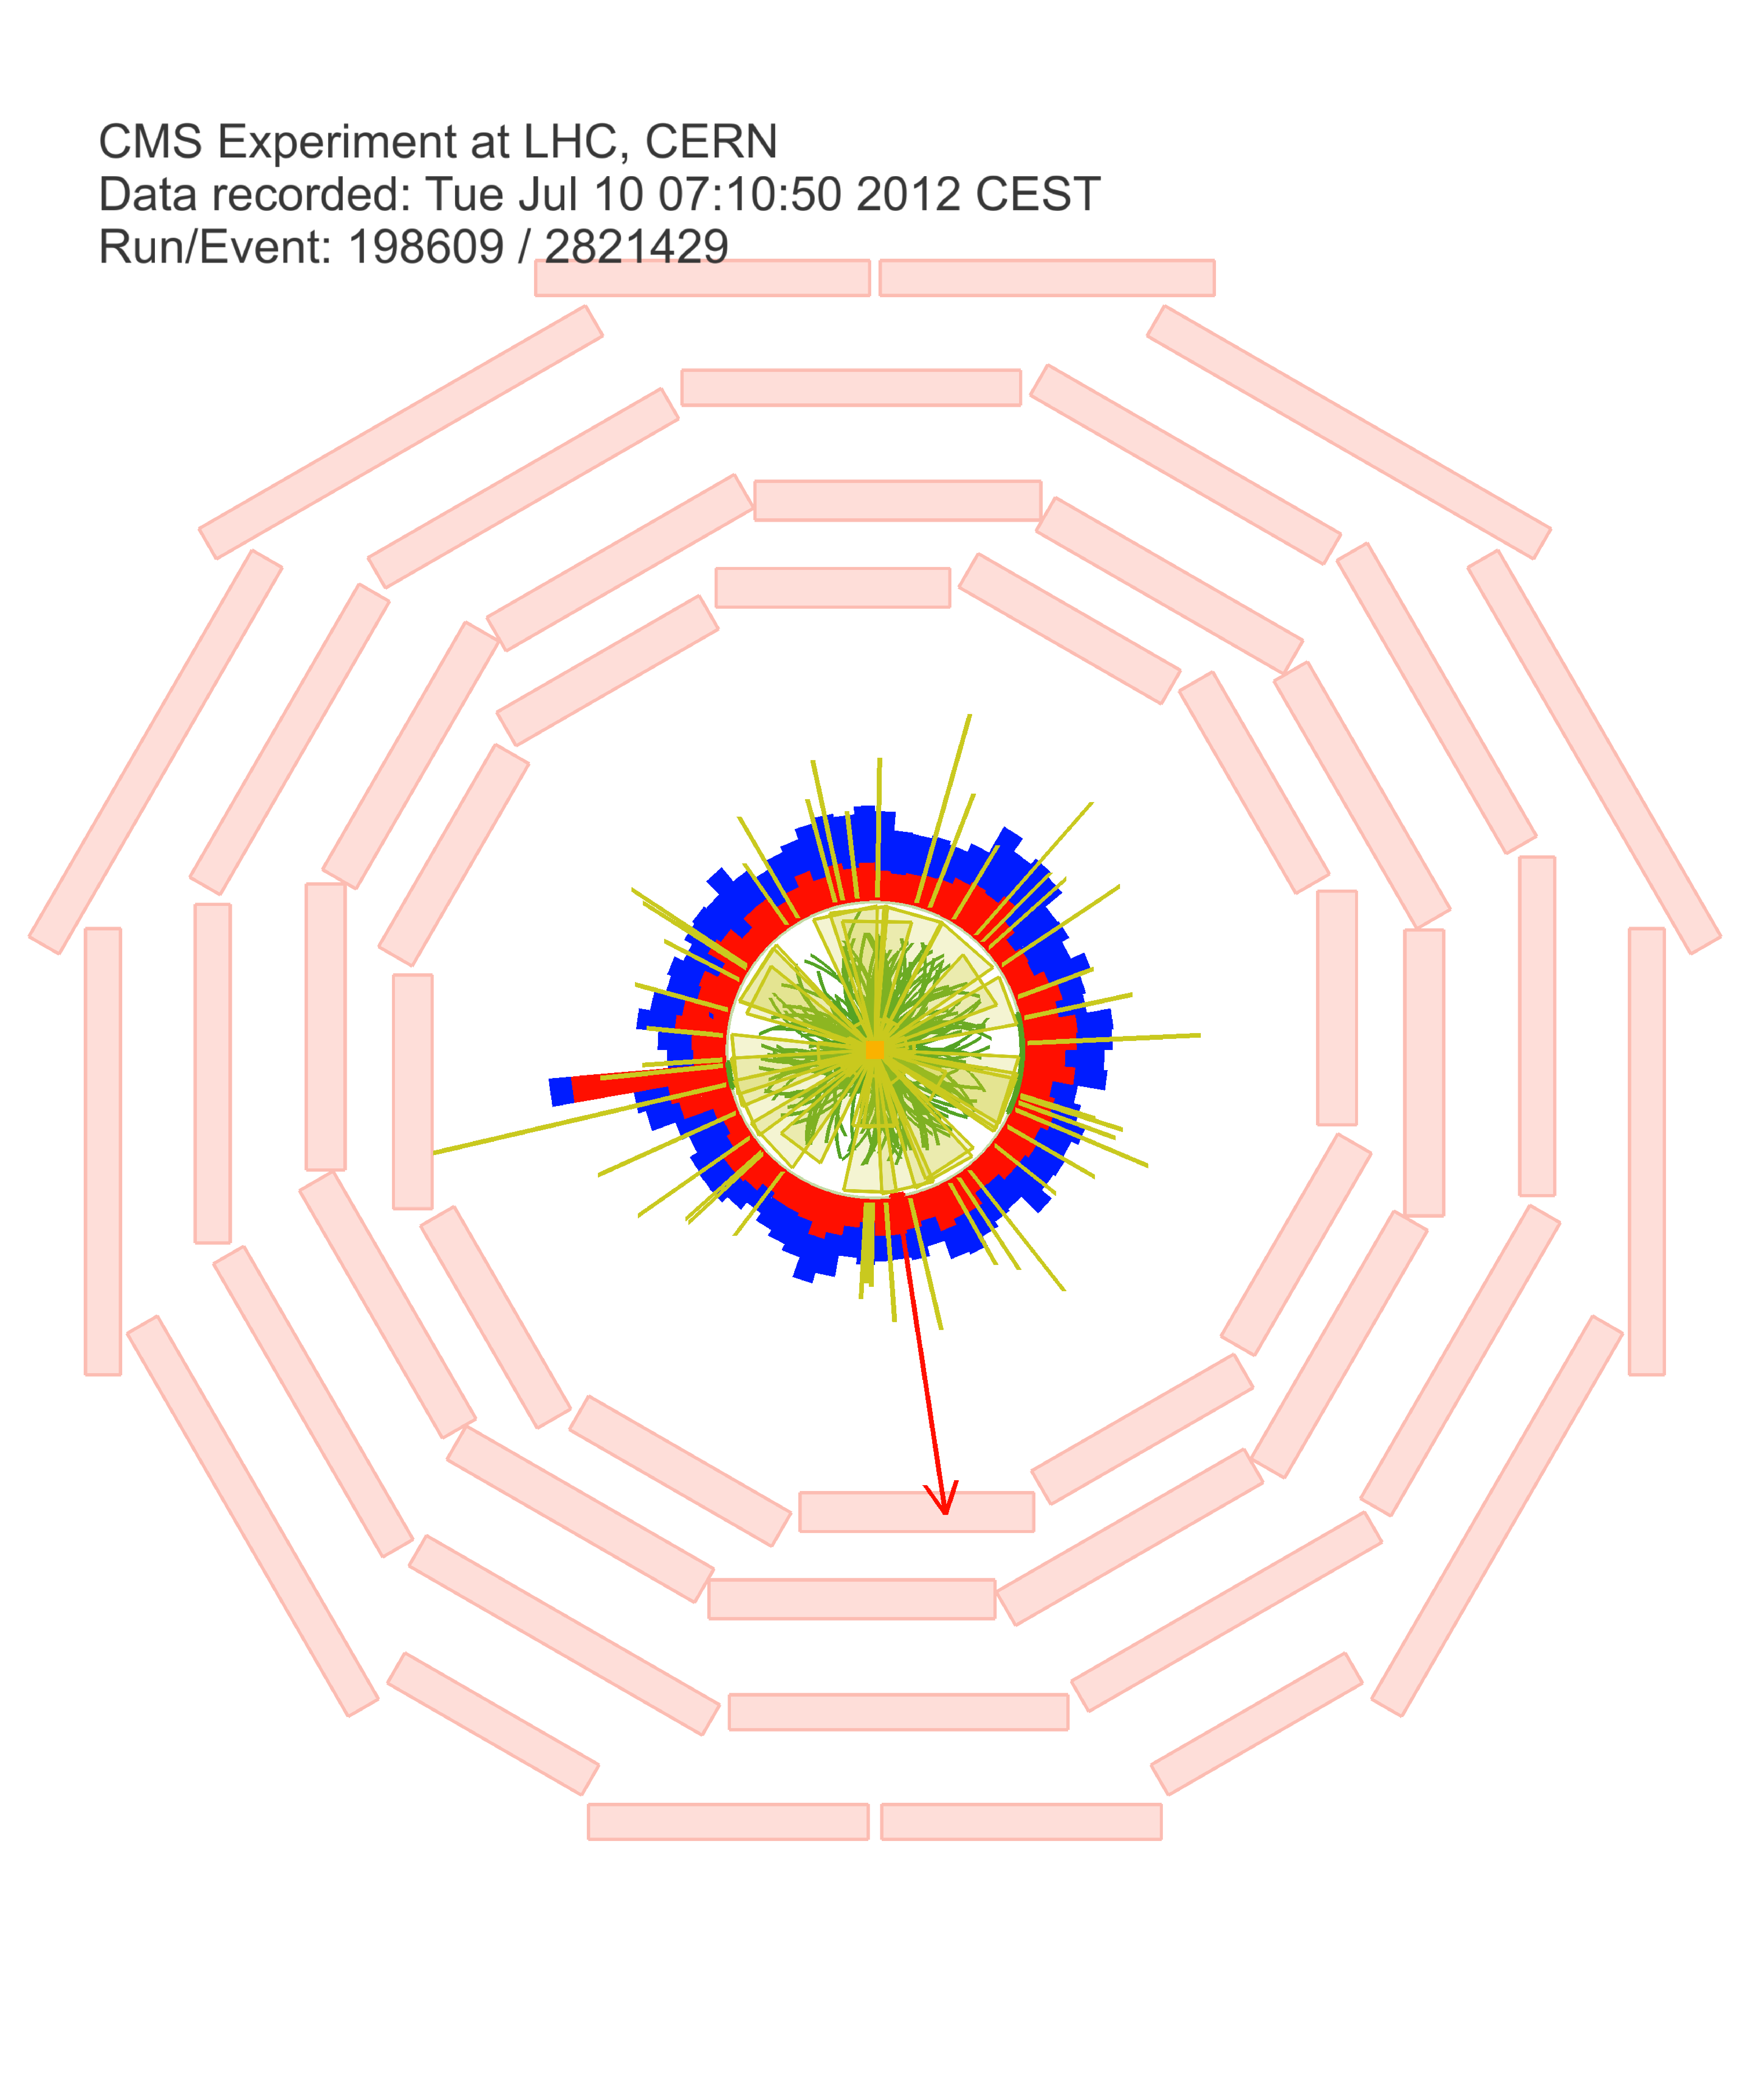
\includegraphics[width=1.6in]{wenu_reco}\label{fig:elestream_before}}
    \subfigure[]{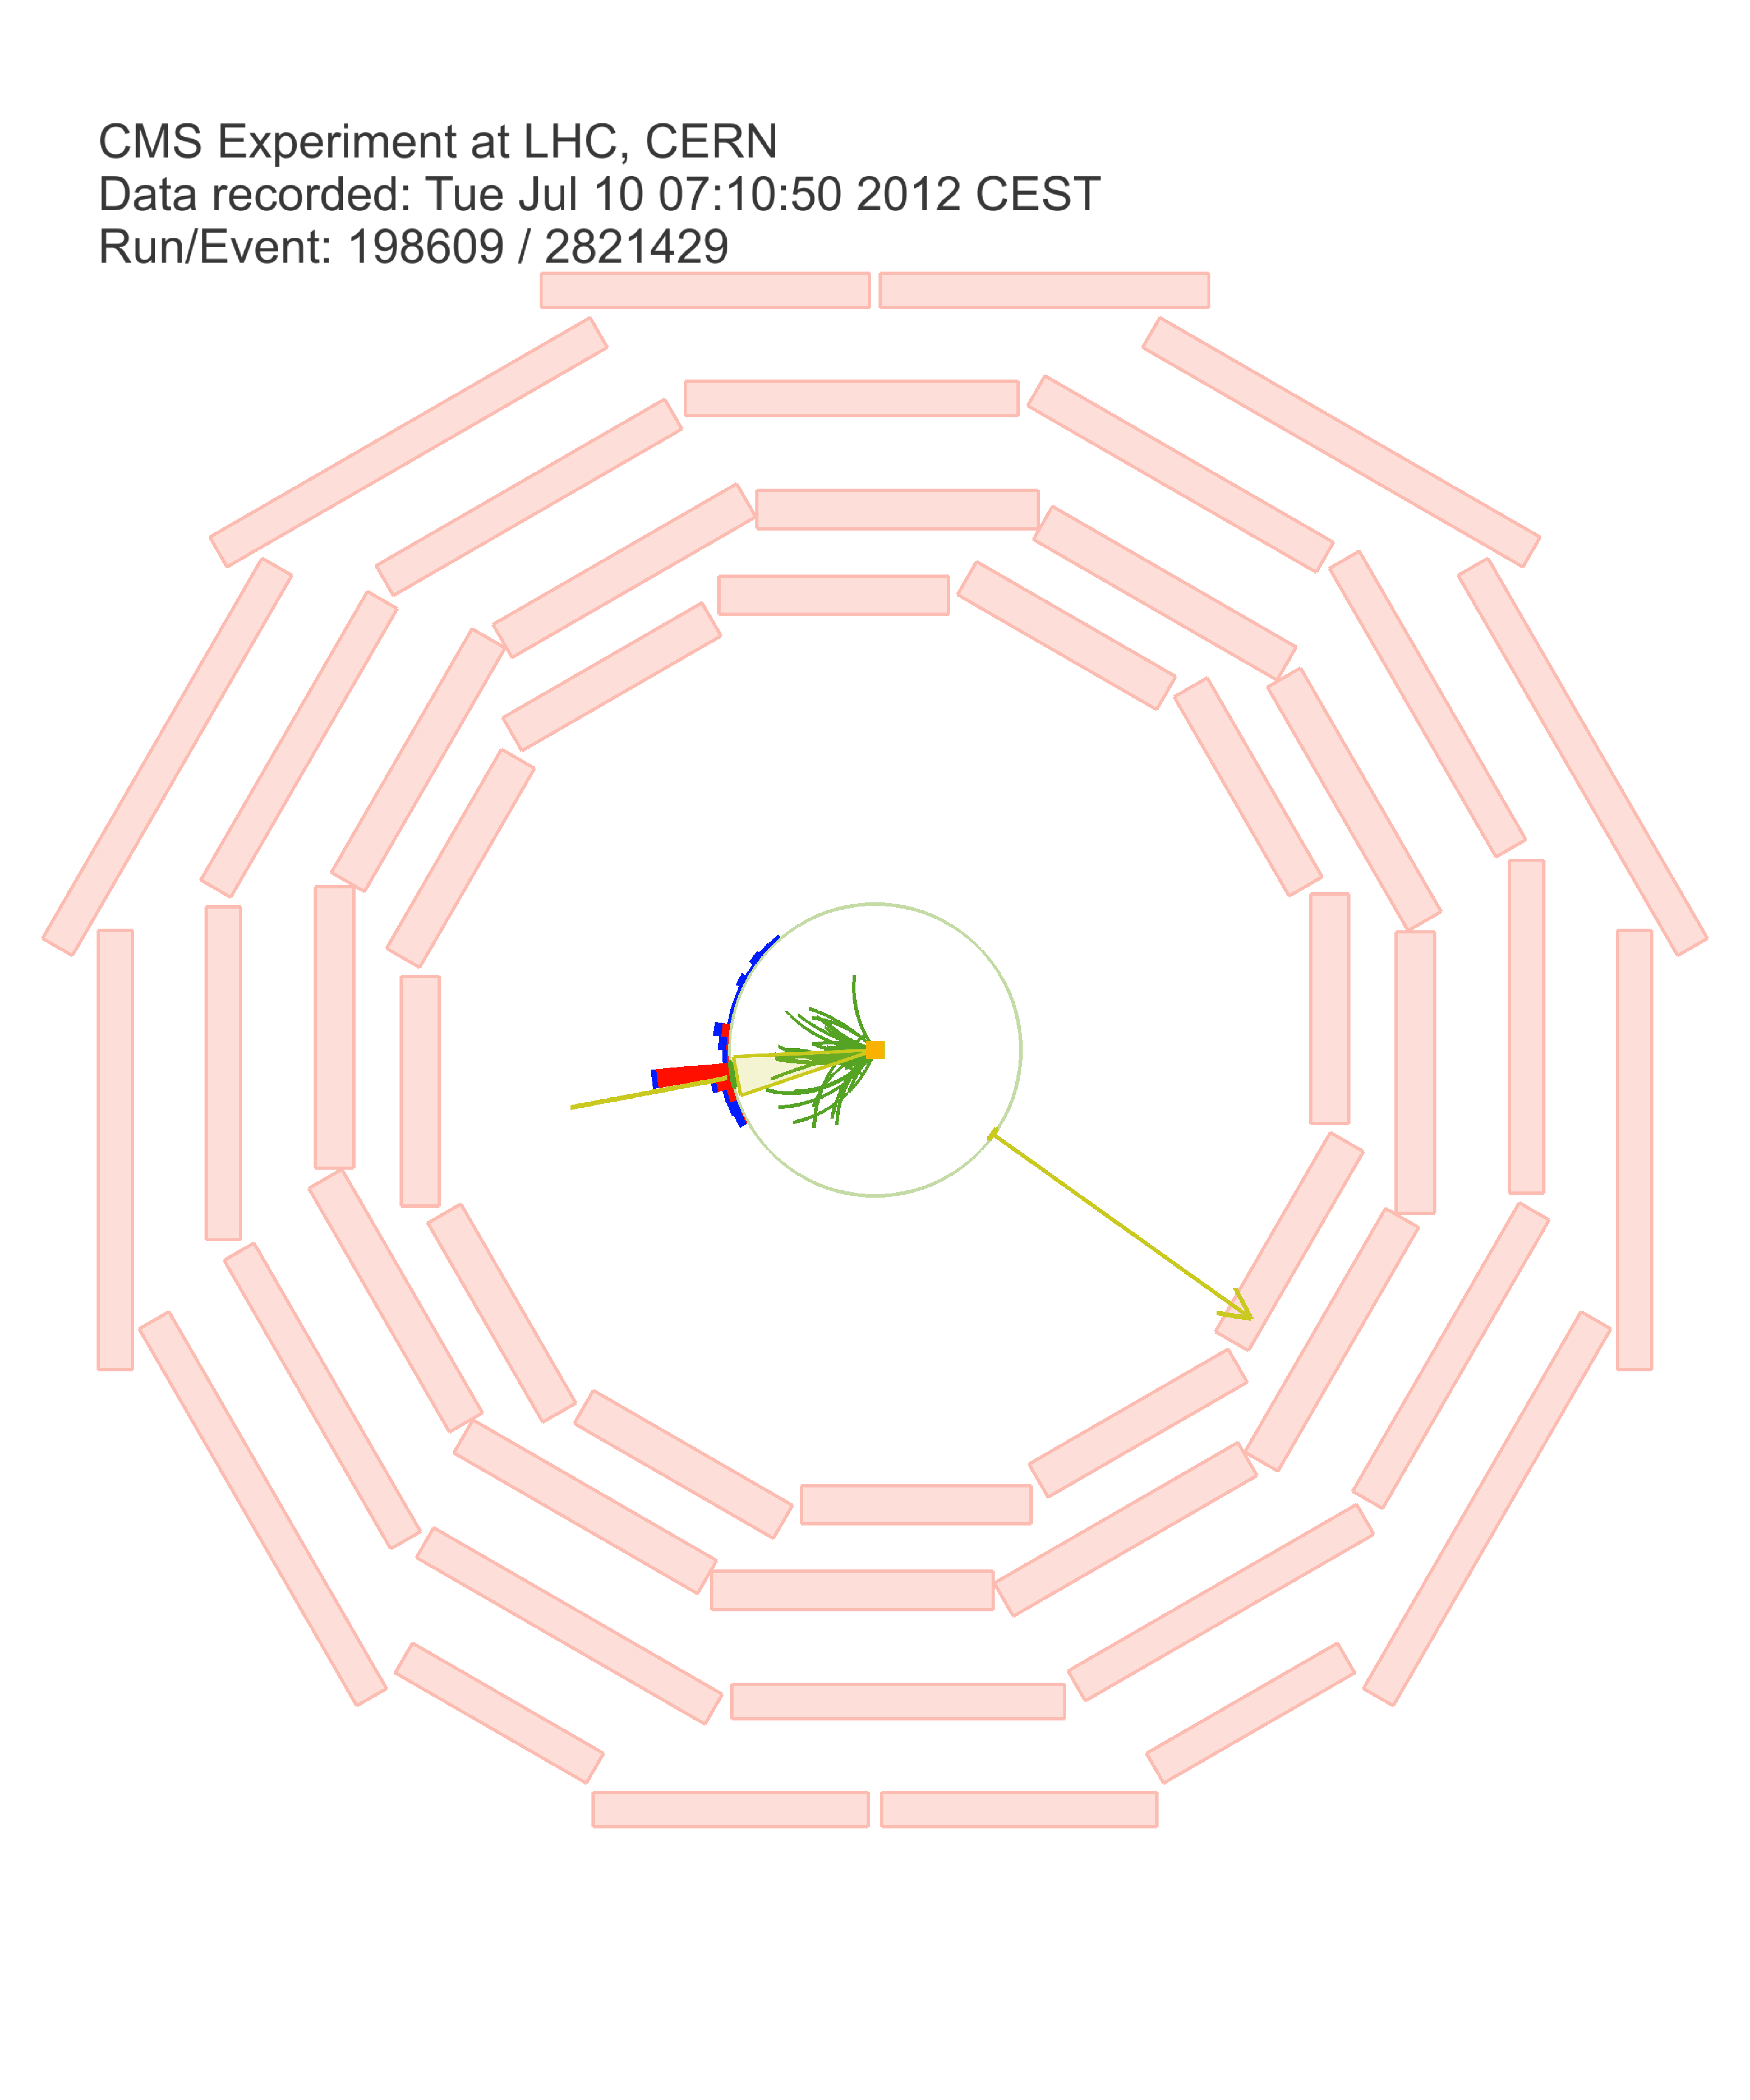
\includegraphics[width=1.6in]{wenu_stream}\label{fig:elestream_after}}
    \caption{Event displays of a $W\to e\nu$ event reconstructed offline, with the full event content (a) and after the event content has been stripped to save only the hits around the electron (a). On Fig. (a), the red arrow shows the reconstructed $\ETslash$, on Fig. (b), the yellow arrow shows the $\ETslash$ as estimated by the HLT objects. \label{fig:elestream}}
  \end{center}
\end{figure}
%


\subsection{Intercalibrations and energy scale}
\label{sec:intercalibrations}
The relative calibration (“intercalibration” IC) is obtained in situ employing collision data, after applying the LC, with different methods employing, the azimuthal symmetry of the energy flow (``$\phi$-symmetry''), photons pairs from the $\pi^0$ decay, and isolated electrons ($E/p$).

The $\phi$-symmetry is based on the equalization of the average energy measured in the different channels placed at the same $\eta$. It employs a dedicated data streams with a very reduced event information allowing to store a high rate of events ($\sim$ 1.5 kHz), and it reaches for each LHC fill cycle a statistical accuracy better than 0.2\% (0.4\%) in the barrel (endcap). The accuracy of the method is indeed limited to few percents by the systematic related to the uncertainty in the knowledge of the material in front of ECAL. Since the systematic does not varies with time the method can be used to track possible time dependencies of the IC values. Indeed in 2012 a drift of the ICs was observed compatible with the imperfection of the LC due to the spread of the value of $\alpha$ in the equation 2. For 2015 a reoptimization of the thresholds is foreseen in order to cope with the different signal / noise ratio. This stream is not expected to be degraded by the higher pile-up, since a larger number of interactions per BX corresponds to a higher rate of minimum bias events available for this calibration method.

The $\pi^0$ mass method is based on the reconstruction of the peak in the spectrum of the invariant mass of unconverted photon pairs due to $\pi^0$ and $\eta$ decays. The photons are reconstructed as $3 \times 3$ matrices of calorimeter channels, and an iterative method is used to determine the IC value of each single channel. It employs a dedicated data streams at high rate( $\sim$ 7 kHz) and it reaches a 0.5\% precision in the central barrel, dominated by systematics when using a data sample corresponding to about 45 days of data taking. In 2015 with the higher pile-up foreseen, the usage of the pile-up subtracted local reconstruction and a new tuning of the selections dependent on $\eta$ are expected to maintain the same precision in the central barrel region and improve it in the regions that were statistically limited in 2012 (in the $\vert\eta\vert\ge2$ only the $\eta\to\gamma\gamma$ was used). Moreover, the usage of particle-flow clusters \cite{CMS:2010eua} will be exploited to benefit from the better cluster calibrations and identification capabilities in the HLT.

The E/p method is based on the comparison of the energy measured in the calorimeter (Eq.\ref{eqn:energy}) to the momentum measured by the tracker for isolated electron, and an iterative procedure is used to extract the IC value for each single channel. The method requires the full 2012 dataset and in the central barrel its precision reaches the systematic limit of 0.5\%, while for $\vert\eta\vert>1$ the statistical contribution is still significant.
These methods may be affected by η dependent systematics due for instance to the effect of pile-up or of the material in front of ECAL, therefore they are employed to obtain a relative calibration of the channels at the same $\eta$ (``$\eta$ ring''), and their results are combined accordingly to their precision. The precision of the different methods and of their combination is reported in Fig.~\ref{fig:intercalib}. In the region $\vert\eta\vert\eta\ge2/5$, above the tracker acceptance, the E/p method can not be used and the high pile-up prevents the reconstruction of the invariant mass peak from $\pi^0$ or $\eta$, therefore only the ICs from the $\phi$-symmetry are available.
To compensate for the imperfection in the LC, the time dependence observed in the ICs from the $\phi$-symmetry method is propagated to the final calibration, in time intervals of the order of one month.
%
\begin{figure}[!t]
  \begin{center}
    \subfigure[]{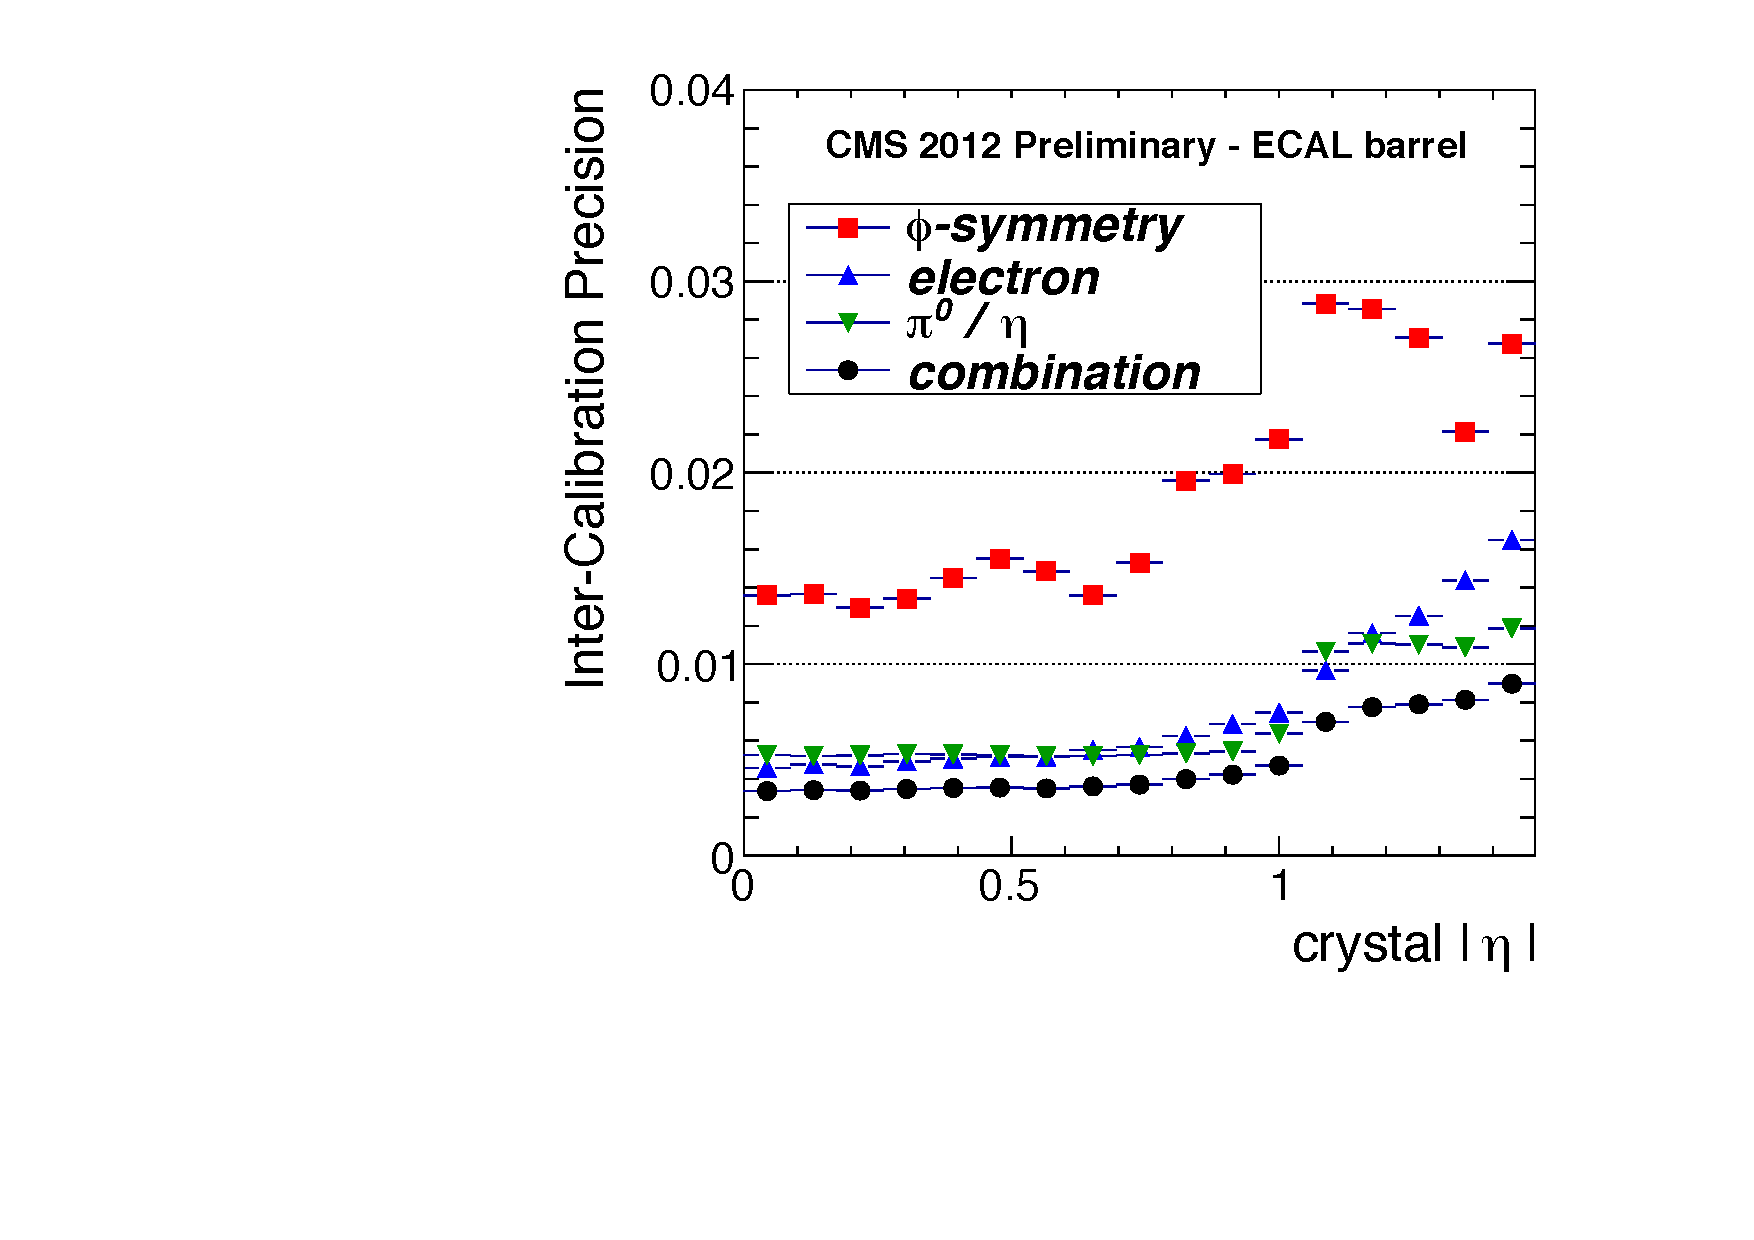
\includegraphics[width=3.0in]{2012EBprecWithCombV3}\label{fig:intercalib_EB}}
    \subfigure[]{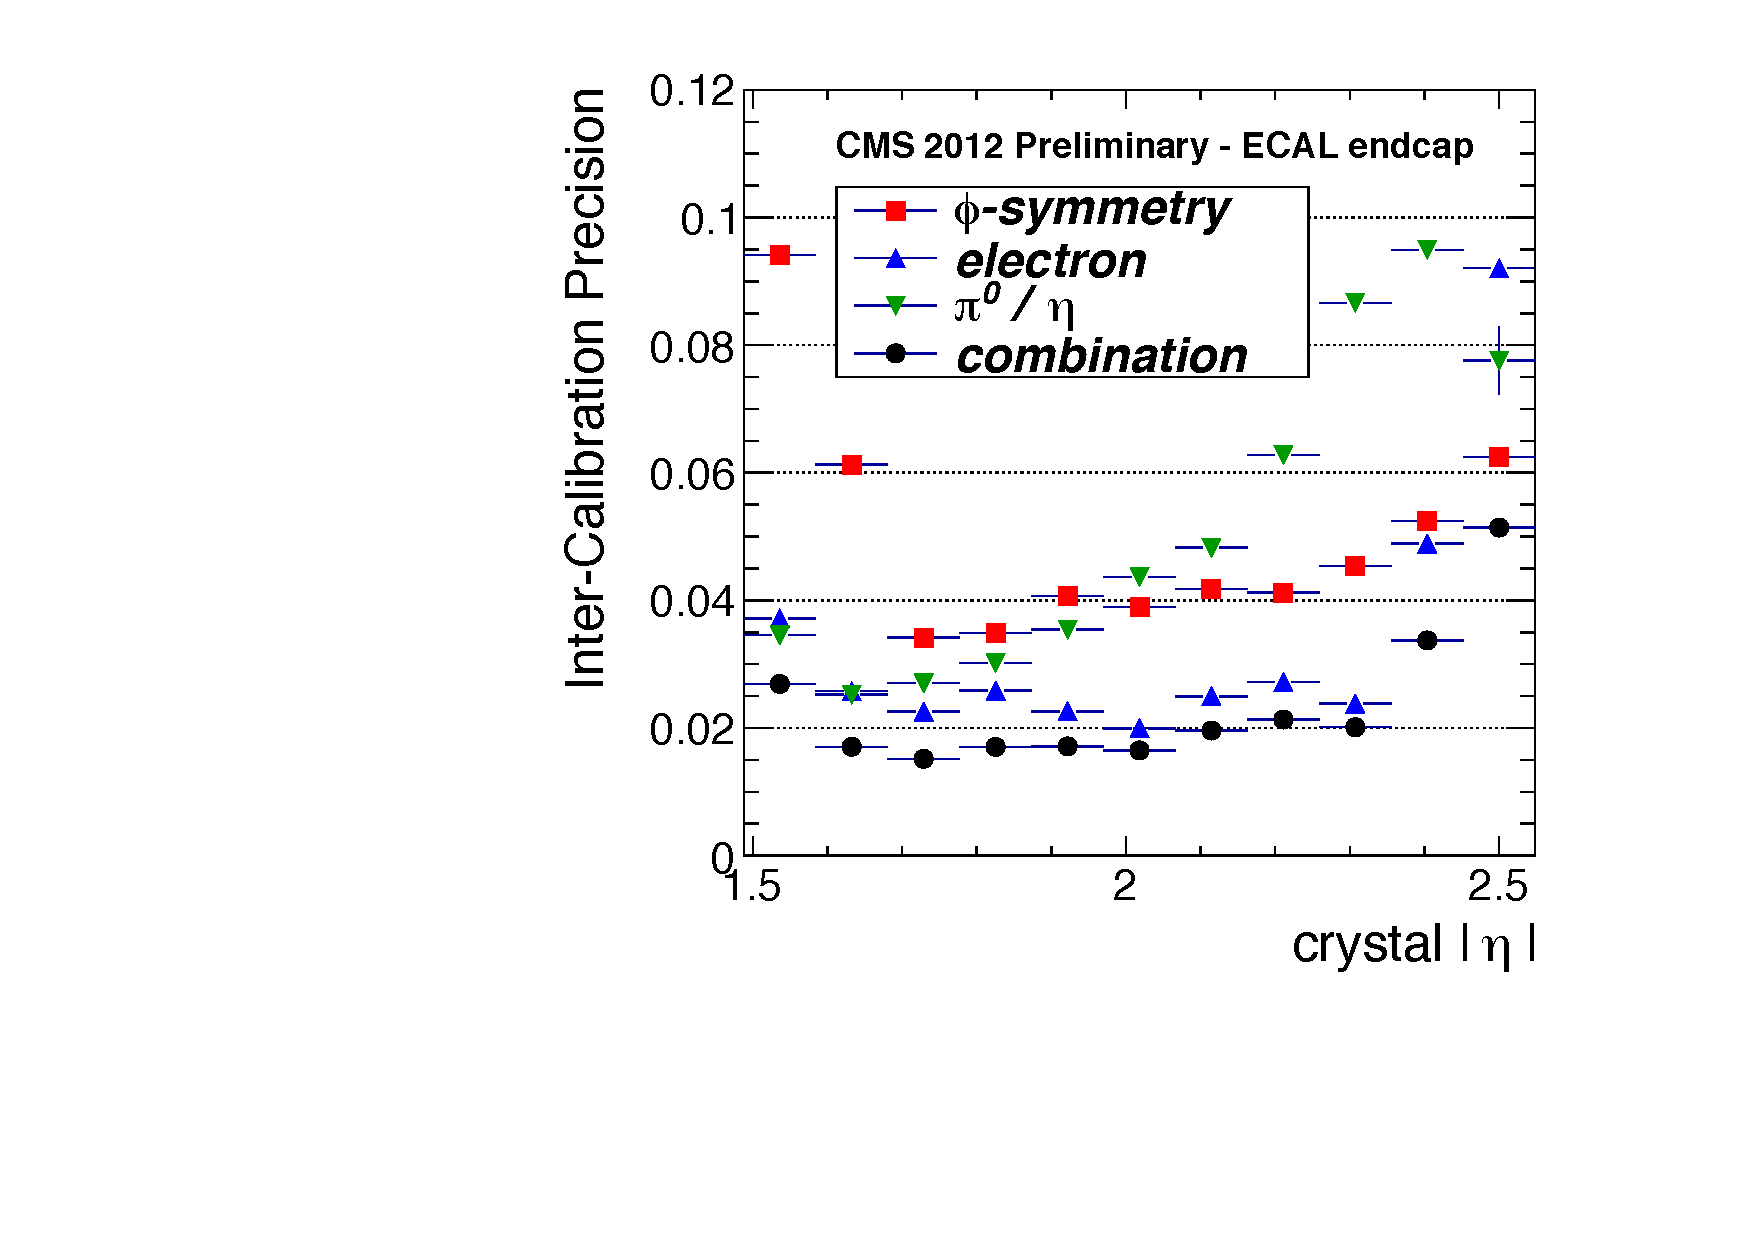
\includegraphics[width=3.0in]{2012EEprecWithCombV3}\label{fig:intercalib_EE}}
    \caption{Precision of the calibration coefficients as a function of $\vert\eta\vert$, for the barrel (a) and the endcaps (b). The precisions of the different methods and of their combination are reported. \label{fig:intercalib}}
  \end{center}
\end{figure}
%

The relative calibration of the $\eta$ rings ($\eta$ scale) is obtained from the peak from the Z boson in the distribution of the invariant mass of electron pairs, selecting a sample of electrons with a low emission of bremsstrahlung. The $\eta$ scale is set to match the expectation from a detailed Monte Carlo simulation of the detector response to pp $\to$ Z $\to e^+e^-$. 

For the LHC Run II the $Z\to ee$ will be also exploited to calibrate the full ECAL employing an invariant mass constraint on the di-electrons. Preliminary studies indicates that this can improve the accuracy of the calibration in the endcap region covered by the tracker and it can also be extended to the region at $\vert\eta\vert>2.5$ by reconstructing one of the two electrons employing only the calorimetric information. In fact even if in this case the effectiveness of the electron identification is reduced it has been shown that the level of background in the invariant mass region close to the Z mass remains marginal.

Finally the overall energy scale $G$ is set, separately for EB and EE, such that the reconstructed Z peak in data matches the one in the Monte Carlo.


\section{Energy resolution and scale}
\IEEEPARstart{T}{he} energy resolution for electrons and photons plays a crucial role in the search for the Higgs with electromagnetic final states, and in particular for the search in the Higgs decays channel H$\to\gamma\gamma$, since it affects the modeling of the expected signal. The accuracy of the calibration directly contributes to the energy resolution with a dilution factor ∼0.7 due to the sharing of the energy among different channels. 

Indeed the actual energy resolution for electrons can be measured from the shape of the invariant mass distribution of electron pairs in the region dominated by $Z\to e^+e^-$ events. Figure \ref{fig:energy_resol_std} reports the measured energy resolution as a function of  $\vert\eta\vert$. The performance with the calibration performed with the full 2012 dataset (blue) can be compared with the one obtained with an initial calibration (grey), and an improvement can be seen in particular in the endcaps. The figure reports also the expected resolution from a Monte Carlo simulation. The discrepancy between data and Monte Carlo measured for electron is propagated to the Monte Carlo simulation of processes involving photons. The tuned energy resolution in the simulation is compared with data in Fig.~\ref{fig:energy_resol_smeared}.  The figures show how the resolution is affected by the amount of material in front of the ECAL and is degraded in the vicinity of the eta cracks between ECAL modules.  Especially in the endcaps, the resolution improves significantly after the calibration using the full 2012 CMS dataset with respect to the prompt calibration from early 2012 CMS data. This conclusion is the proof of the need of regular full calibrations of ECAL also during Run II. 
%
\begin{figure}[!t]
  \begin{center}
    \subfigure[]{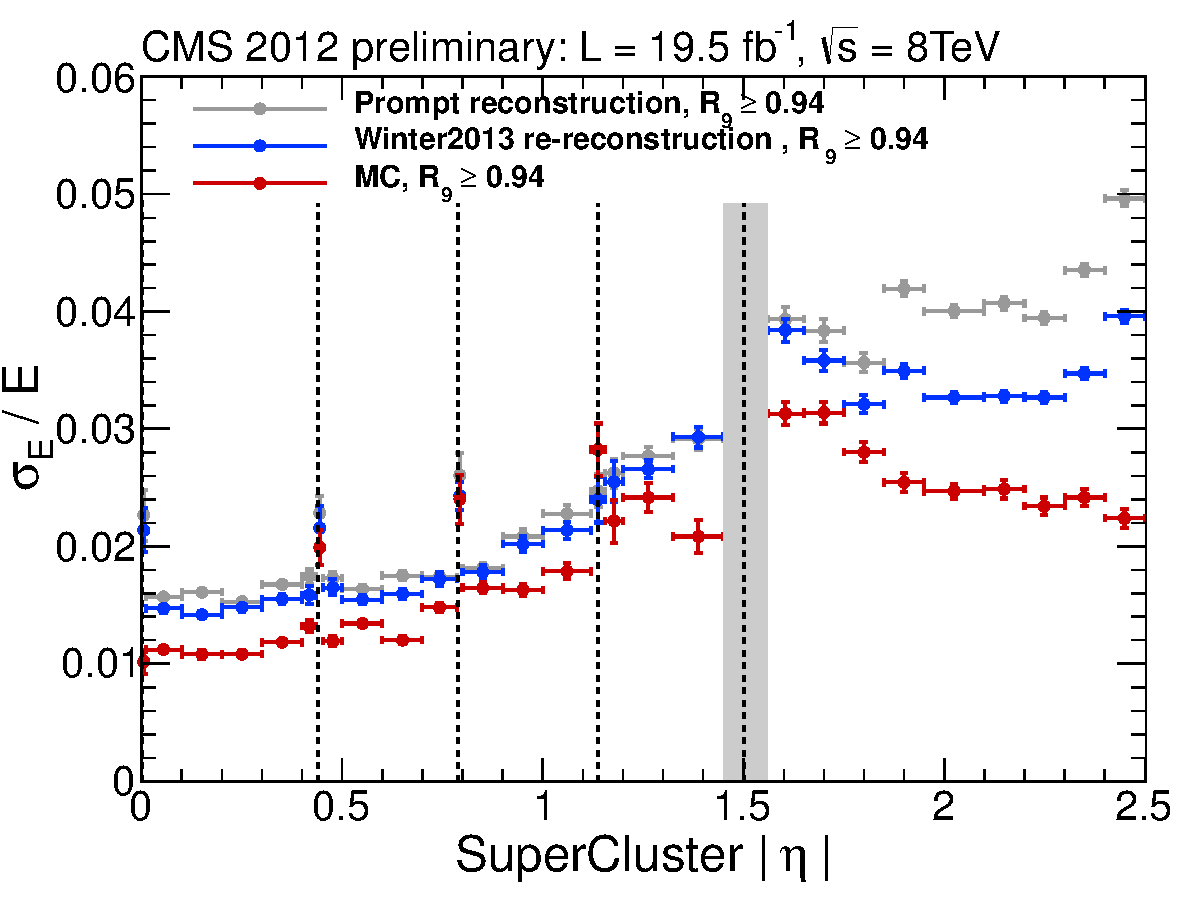
\includegraphics[width=3.0in]{resolution_highR9_beforesmear}\label{fig:energy_resol_std}}
    \subfigure[]{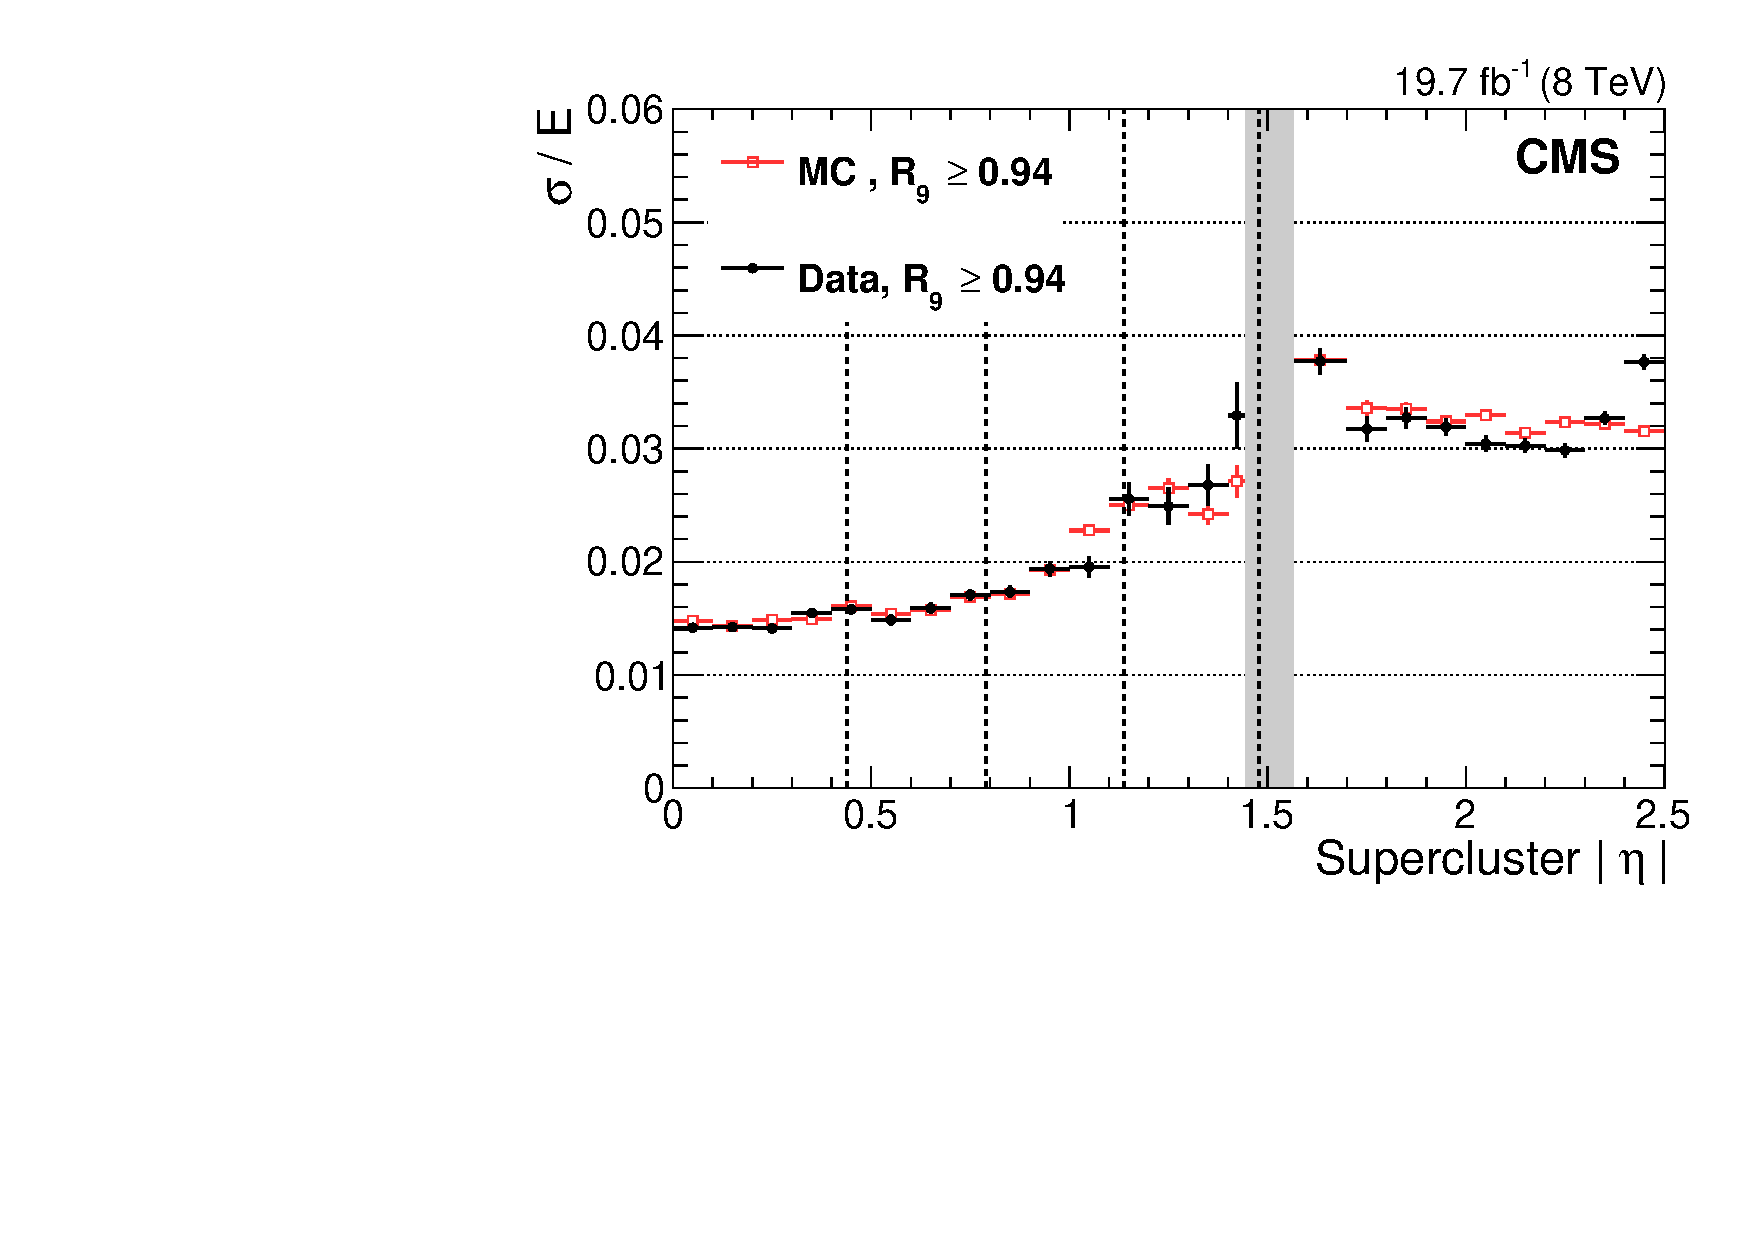
\includegraphics[width=3.0in]{resolution_highR9_aftersmear}\label{fig:energy_resol_smeared}}
    \caption{Relative electron (ECAL) energy resolution unfolded in bins of pseudo-rapidity $\vert\eta\vert$ for the barrel and the endcaps. Electrons from $Z\to ee$ decays are used. The resolution is shown for low bremsstrahlung electrons ($R_9>0.94$ with $R_9 = E_{3 \times 3} / E_{SC}$). For Fig. (a), the plain simulation is used, while in Fig. (b) the tuned simulation is shown. ~\label{energy_resol}}
  \end{center}
\end{figure}
%

For an improved and detailed understanding of the ECAL performances a ``run-dependent'' Monte Carlo simulation have been developed which mimics the evolving conditions, in terms of pile-up, noise due to the radiation-induced increment of the APD dark current in the barrel and crystal transparency. The evolution of the dark current measured for the barrel APDs operated at gain 50 and kept at 18$^\circ$C is shown in Fig.~\ref{fig:idark}. The figure also shows that during technical stops and winter shutdowns a part of the APD defects anneals and the current reduces. The short time component of the annealing is of about 20 days. 
%
\begin{figure}[!t]
  \begin{center}
    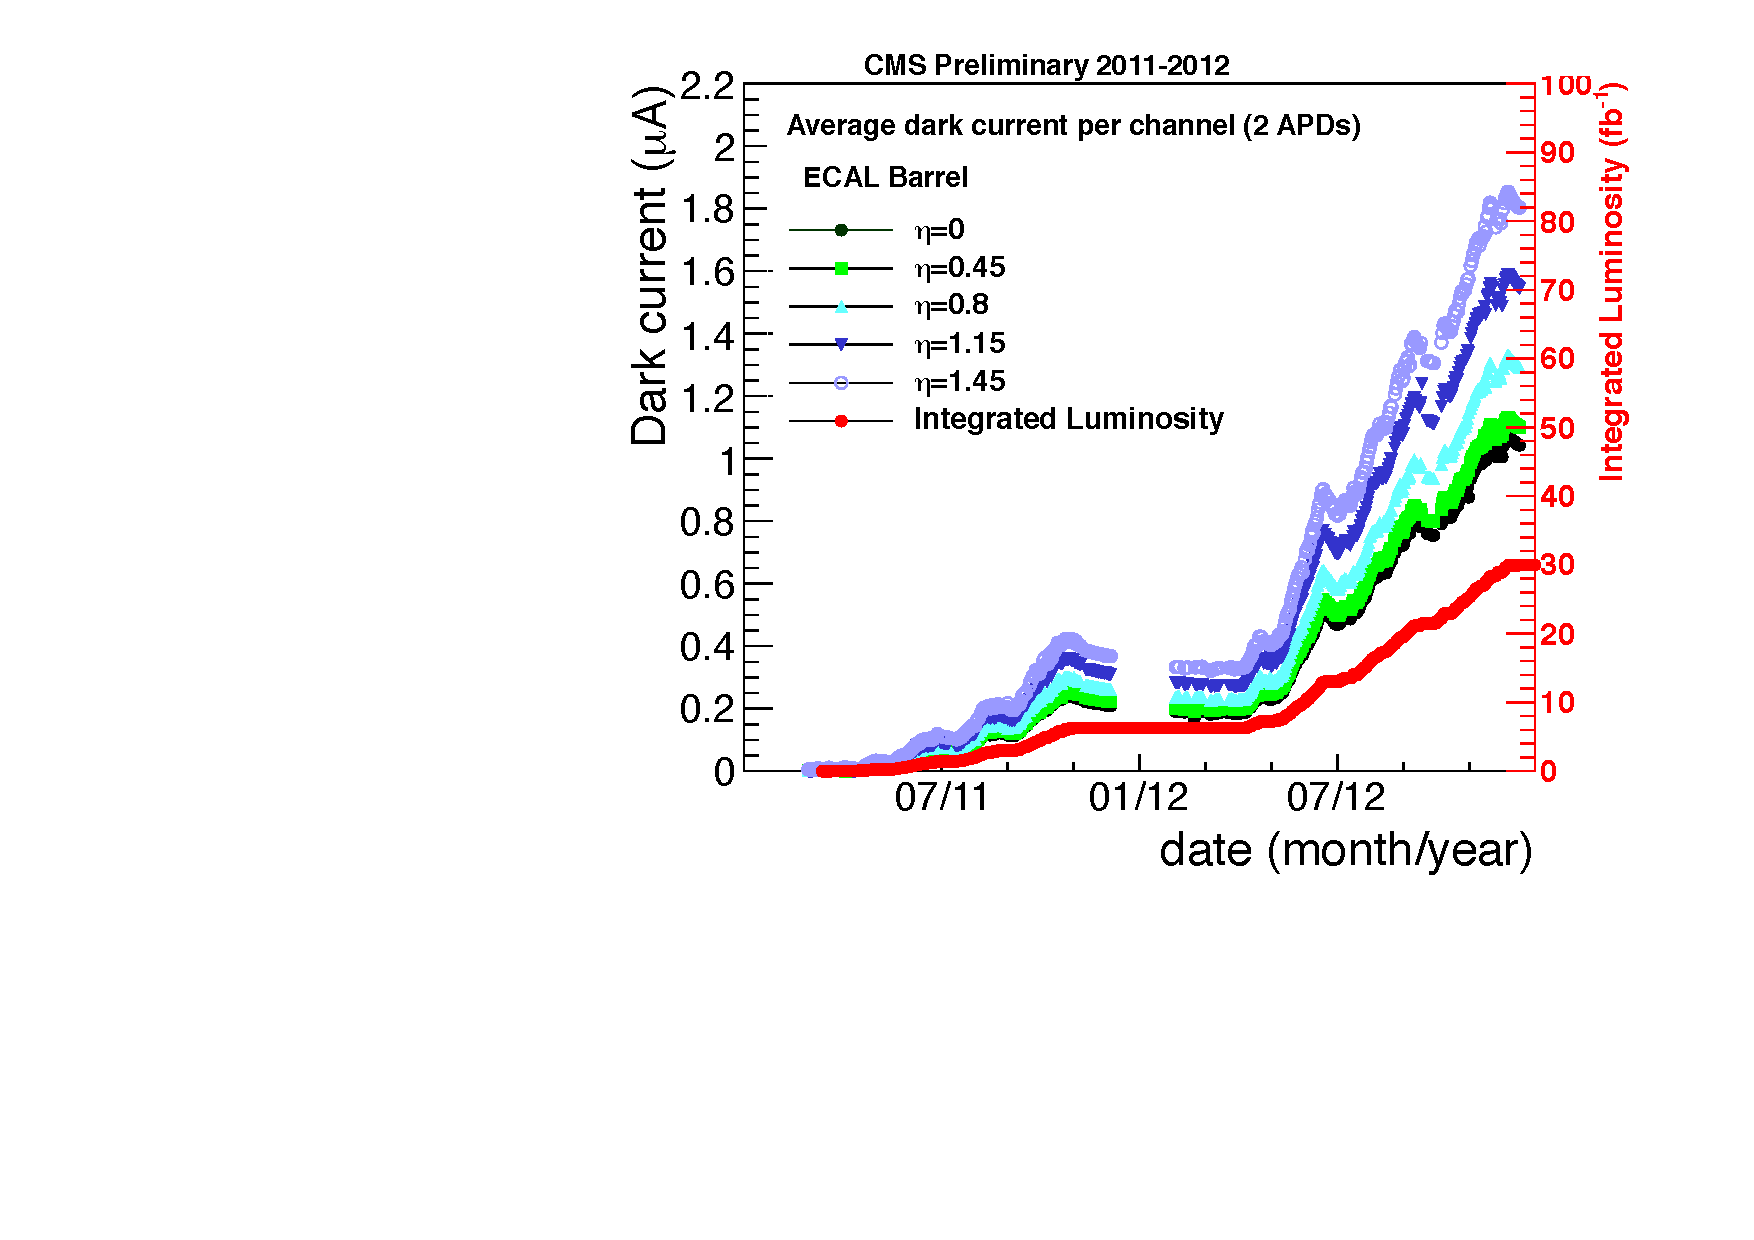
\includegraphics[width=3.3in]{HV_avg_history}
    \caption{Dark current evolution of the Avalanche Photodiodes installed in the ECAL Barrel (2 APDs are installed on each crystal). The plot shows the average dark current measured per channel as a function of time. The colors indicate different eta regions of the ECAL barrel. The delivered luminosity is also shown. \label{fig:idark}}
  \end{center}
\end{figure}
%
The run-dependent Monte Carlo (not shown in Fig.~\ref{energy_resol}) has been used to derive the results of the search of the Higgs bosons in the decay channel H$\to\gamma\gamma$, and it is now implemented as the default one for the Run II simulations. 

Moreover, with the LHC Run I data it has been possible to improve the measurement of the amount of material in front of the ECAL, mostly the tracker and its services. Methods use the energy loss of charged tracks, the energy loss of electrons, the comparison between collisions taken with and without magnetic field, and the ratio between the energy deposits in the preshower and the corresponding clusters in the endcaps. The results of the independent methods show agreement for the main dependency of the measured over predicted ratio of the material thickness (Fig.~\ref{fig:material}). The charged track and electron methods are then combined to describe in-homogeneities in $\phi$ of the tracker services, and are included in the simulation for the Run II data taking.
%
\begin{figure}[!t]
  \begin{center}
    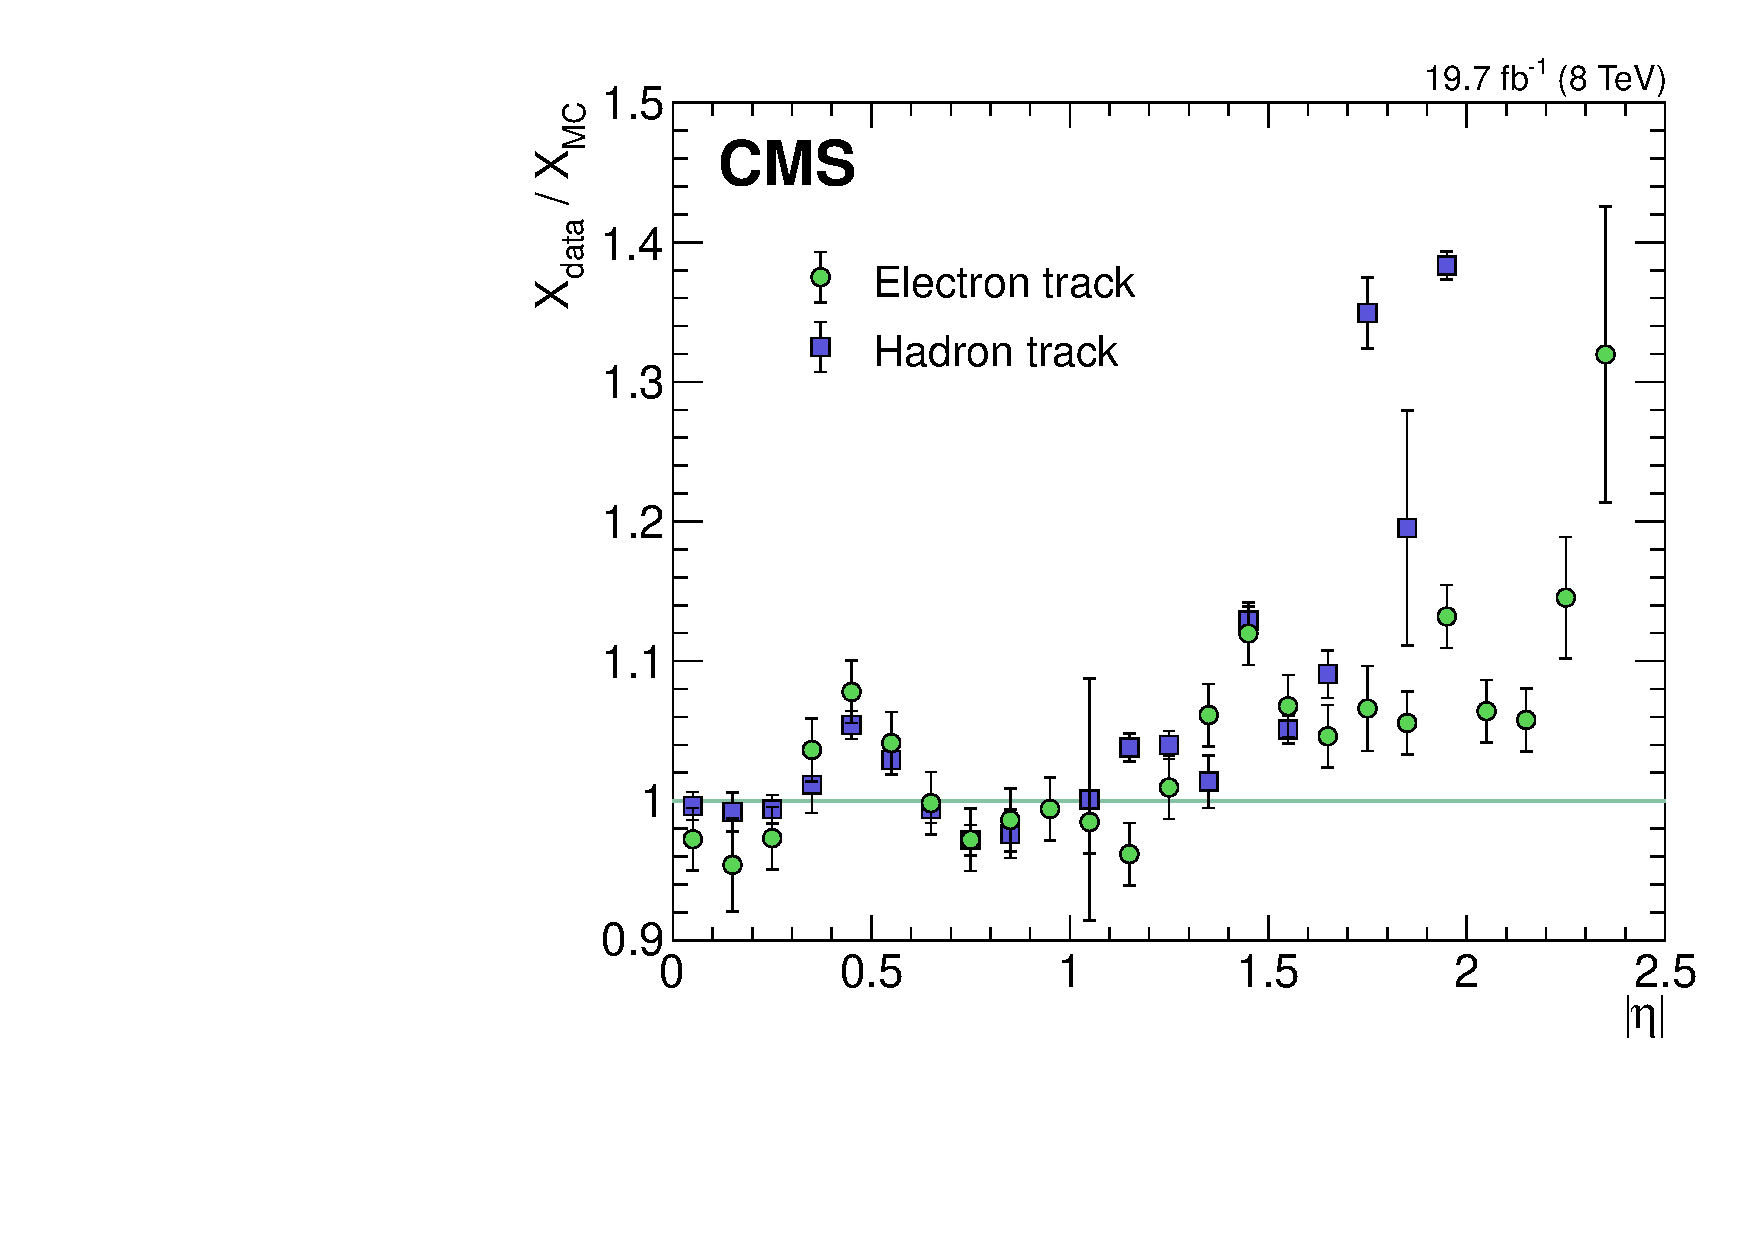
\includegraphics[width=3.0in]{material}
    \caption{Tracker material thickness (in terms of radiation lengths) estimated in the data, $X_\mathrm{data}$, relative to that estimated in simulated events, $X_\mathrm{MC}$, as a function of $\vert\eta\vert$, using electrons in $Z\to ee$ events (circles), and low momentum charged hadrons (squares). \label{fig:material}}
  \end{center}
\end{figure}
%


\section{Time reconstruction}
\label{sec:timereco}
\IEEEPARstart{T}{he} scintillation decay time of the crystals is comparable to the LHC bunch crossing interval of 25 ns, and about 80\% of the light is emitted in 25 ns. This allows excellent time resolution. The time of each ECAL hit can be measured through the ratios of the consecutive 10 digitized samples of the pulse shape. The two alternative representations of the pulse shape are shown in Fig.~\ref{fig:pulse_shapes_funcs}: the amplitude as a function of the difference between the time of the ADC sample ($T$) and the time of the maximum of the pulse ($T_{\rm max}$) and the time difference $T-T_{\rm max}$ as a function of the ratio of the amplitudes in two consecutive samples. The latter is used for the time estimate \cite{Chatrchyan:2009aj}.  
%
\begin{figure}[!t]
  \begin{center}
    \subfigure[]{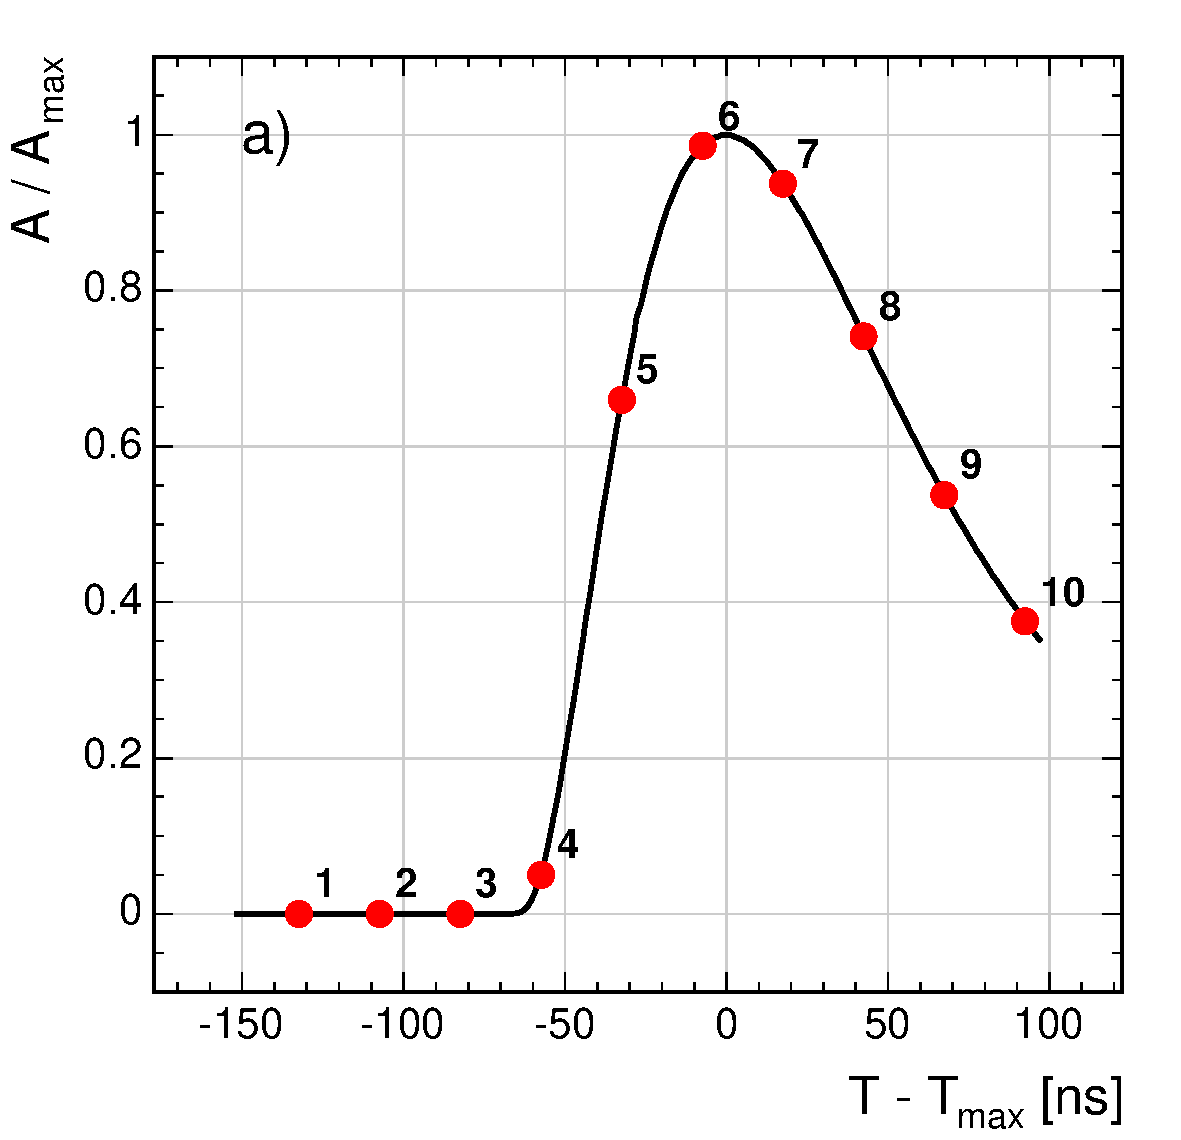
\includegraphics[width=1.7in]{pulseshape}\label{fig:pulse_shapes_normal}}
    \subfigure[]{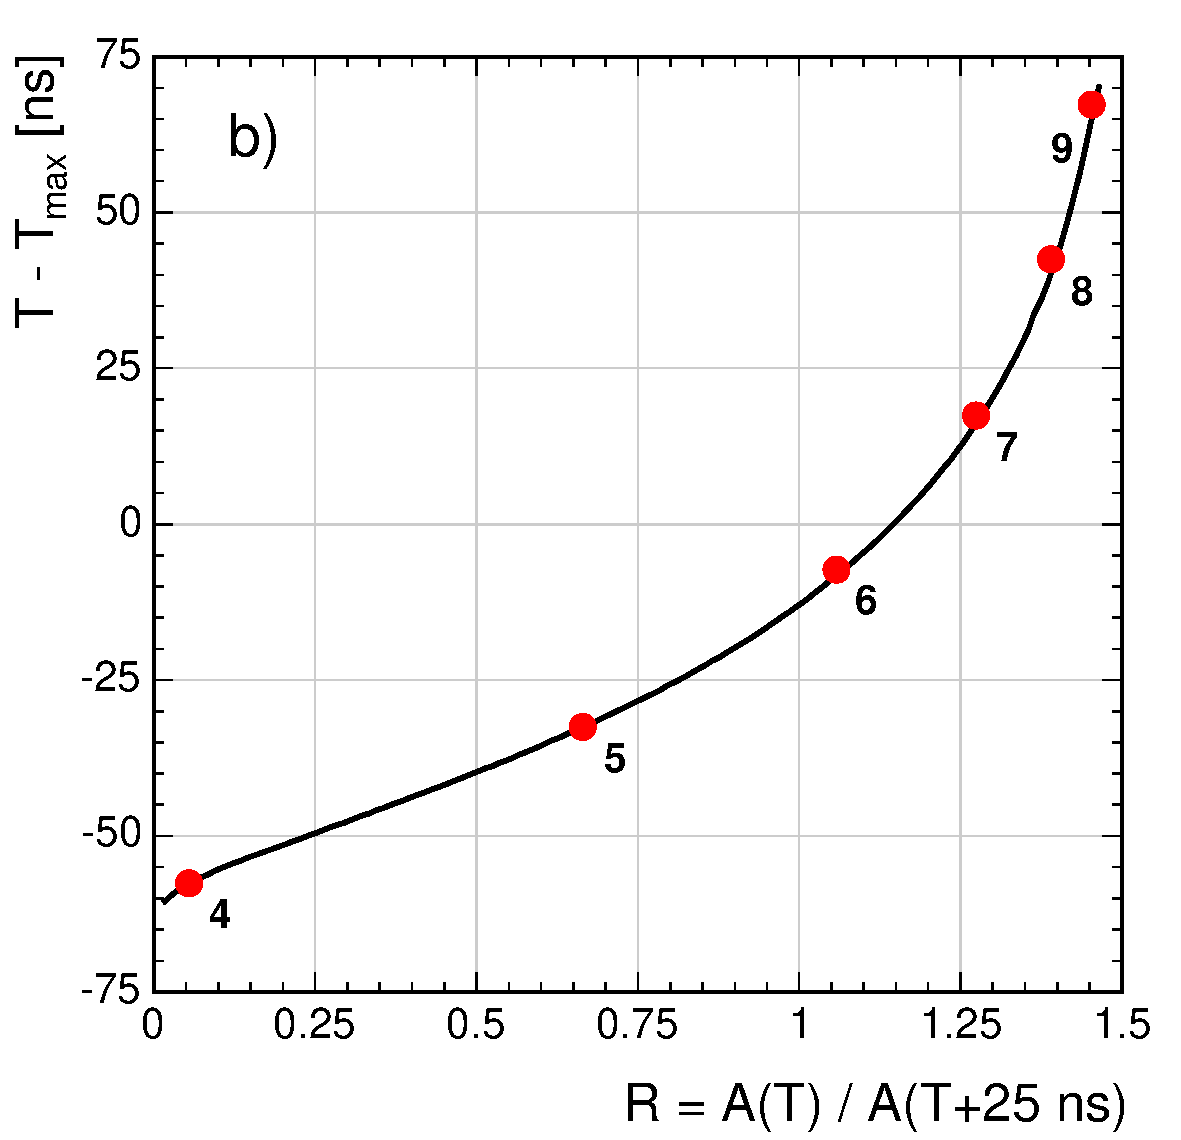
\includegraphics[width=1.7in]{ratio}\label{fig:pulse_shapes_ratio}}
    \caption{Typical ECAL pulse shape, with the 10 discrete samples shown as dots, as a function of $T-T_{\rm max}$, defined in the text (a). The pedestal has been subtracted and the samples normalized to the maximum amplitude. The solid line is the average pulse shape, as measured with a beam of electrons triggered asynchronously with respect to the digitizer clock phase. (b): Pulse shape representation using $T-T_{\rm max}$ as a function of the ratio of the amplitudes in two consecutive samples ($R$). \label{fig:pulse_shapes_funcs}}
  \end{center}
\end{figure}
%

The stability of the time measurement required to maintain the energy resolution is on the order of 1 ns. The better the precision of time measurement and synchronization, the larger the rejection of backgrounds with a broad time distribution. Such backgrounds are out-of-time proton-proton interactions, cosmic rays, beam halo muons, and electronic noise. Precise time measurement also makes it possible to put constraints on the presence of long-lived particles predicted by models beyond the Standard Model decaying into photons which reach the ECAL  out-of-time with respect to particles traveling at the speed of light from the interaction point. To achieve these goals the time measurement performance both at low energy (1 GeV or less) and high energy (several tens of GeV for showering photons) becomes relevant.
The time reconstruction algorithm is in general degraded when more than one overlapping pulse is present.  For the high energy pulses, relevant to the beyond Standard Model signals, the low occupancy of pile-up particles in the same crystal with a competing energy will be still small in Run II, thus the same algorithm is foreseen to be used in 2015.


\section{Time resolution measurement}
\label{sec:timeresolution}
\IEEEPARstart{T}{he} time resolution is extracted by comparing the time measured in ECAL hits which are, or can be made, synchronous. Two methods are used to measure it on collision data.

The first method compares the time of the two electrons of a Z decay. The time of the electron corresponds to the one of the most energetic hit of the SC. The time is corrected by the time-of-flight of the electrons, which is determined from the primary vertex position, obtained from the electron tracks. The two SCs are required to have a seed cluster satisfying loose criteria on the shape of the deposit and the resulting invariant mass has to be consistent with the Z boson mass (60 GeV $<m_{ee}<$ 150 GeV). The energy of each of the two hits must fulfill 10 GeV $<E<$ 120 GeV. The resolution is extracted as the $\sigma$ parameter of a Gaussian fit to the core of the time difference distribution. Figure \ref{fig:time_resol_zee} shows the resulting resolution is studied as a function of the effective amplitude, which depends on the amplitudes measured in the two crystals as $A_{\rm eff} = A_1 A_2 \sqrt{A_1^2 + A_2^2}$. The noise term is very similar to the one obtained in electron beam test and the constant term is estimated be $\approx$ 150 ps. This value is much better then the one needed to achieve the best energy resolution (1 ns), but it is still far from the test beam one, which was about 20 ps.

The second method compares the two most energetic neighboring crystals of a photon cluster, with a similar amount of energy. The second requirement is to minimize the shower propagation effects. Additional selection criteria are applied, based on the shape of the ECAL cluster and on the energy of the ECAL hit (E $<$ 120 GeV). The resulting resolution, as a function of the effective amplitude, shows a smaller constant term, of about 70 ps, closer to the test beam results. The resulting function is shown in Fig.~\ref{fig:time_resol_neighbors}.

%
To further investigate the difference a study is performed, comparing crystals belonging to either the same or different readout units. The readout unit corresponds to a trigger tower which is a $5 \times 5$ matrix of crystals.  The different constant term obtained in the two cases, 67 ps vs 130 ps, does not explain the difference with respect to the test beam results but indicates that there are effects related to the clock distribution to the individual readout units, more than a residual timing jitter. This hypothesis will be further investigated with future studies.
%
\begin{figure}[!t]
  \begin{center}
    \subfigure[]{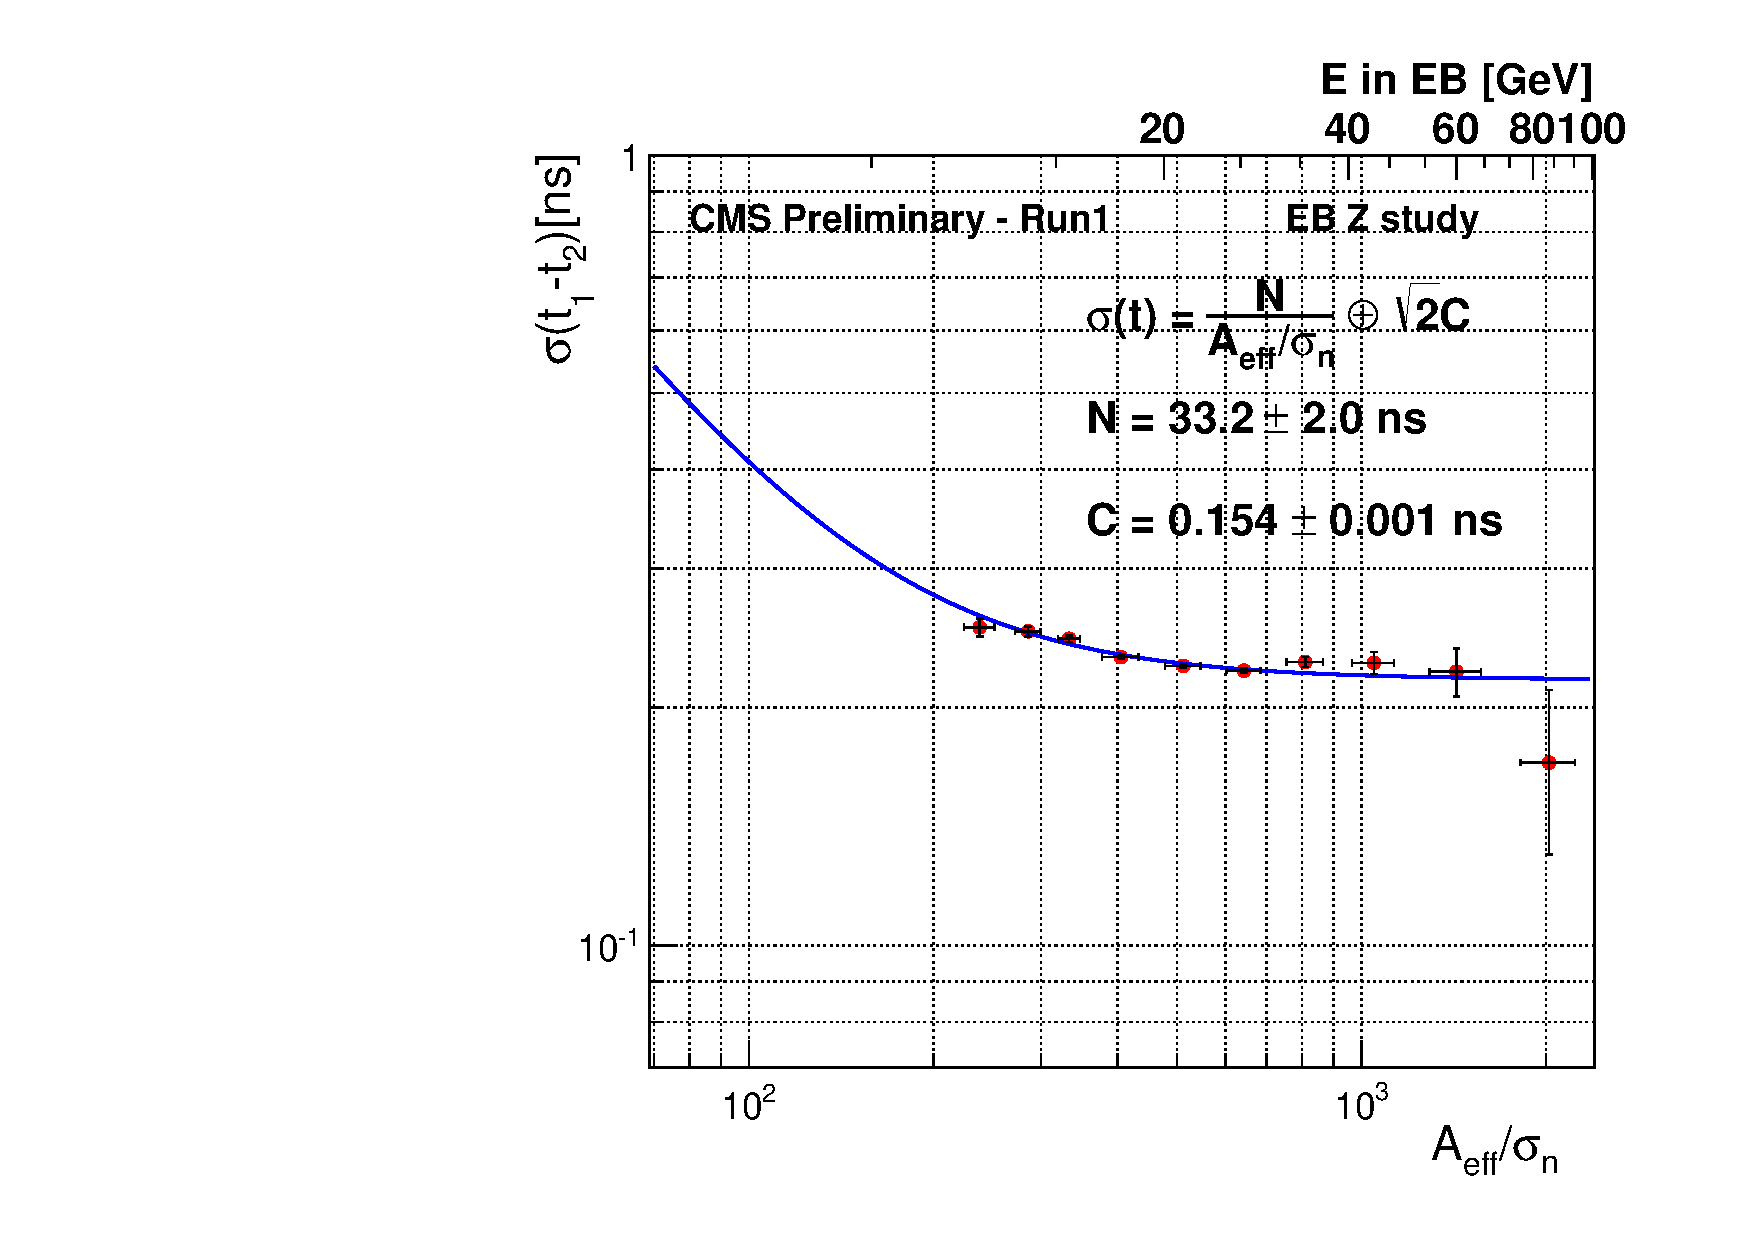
\includegraphics[width=3.0in]{time_resol_Z}\label{fig:time_resol_zee}}
    \subfigure[]{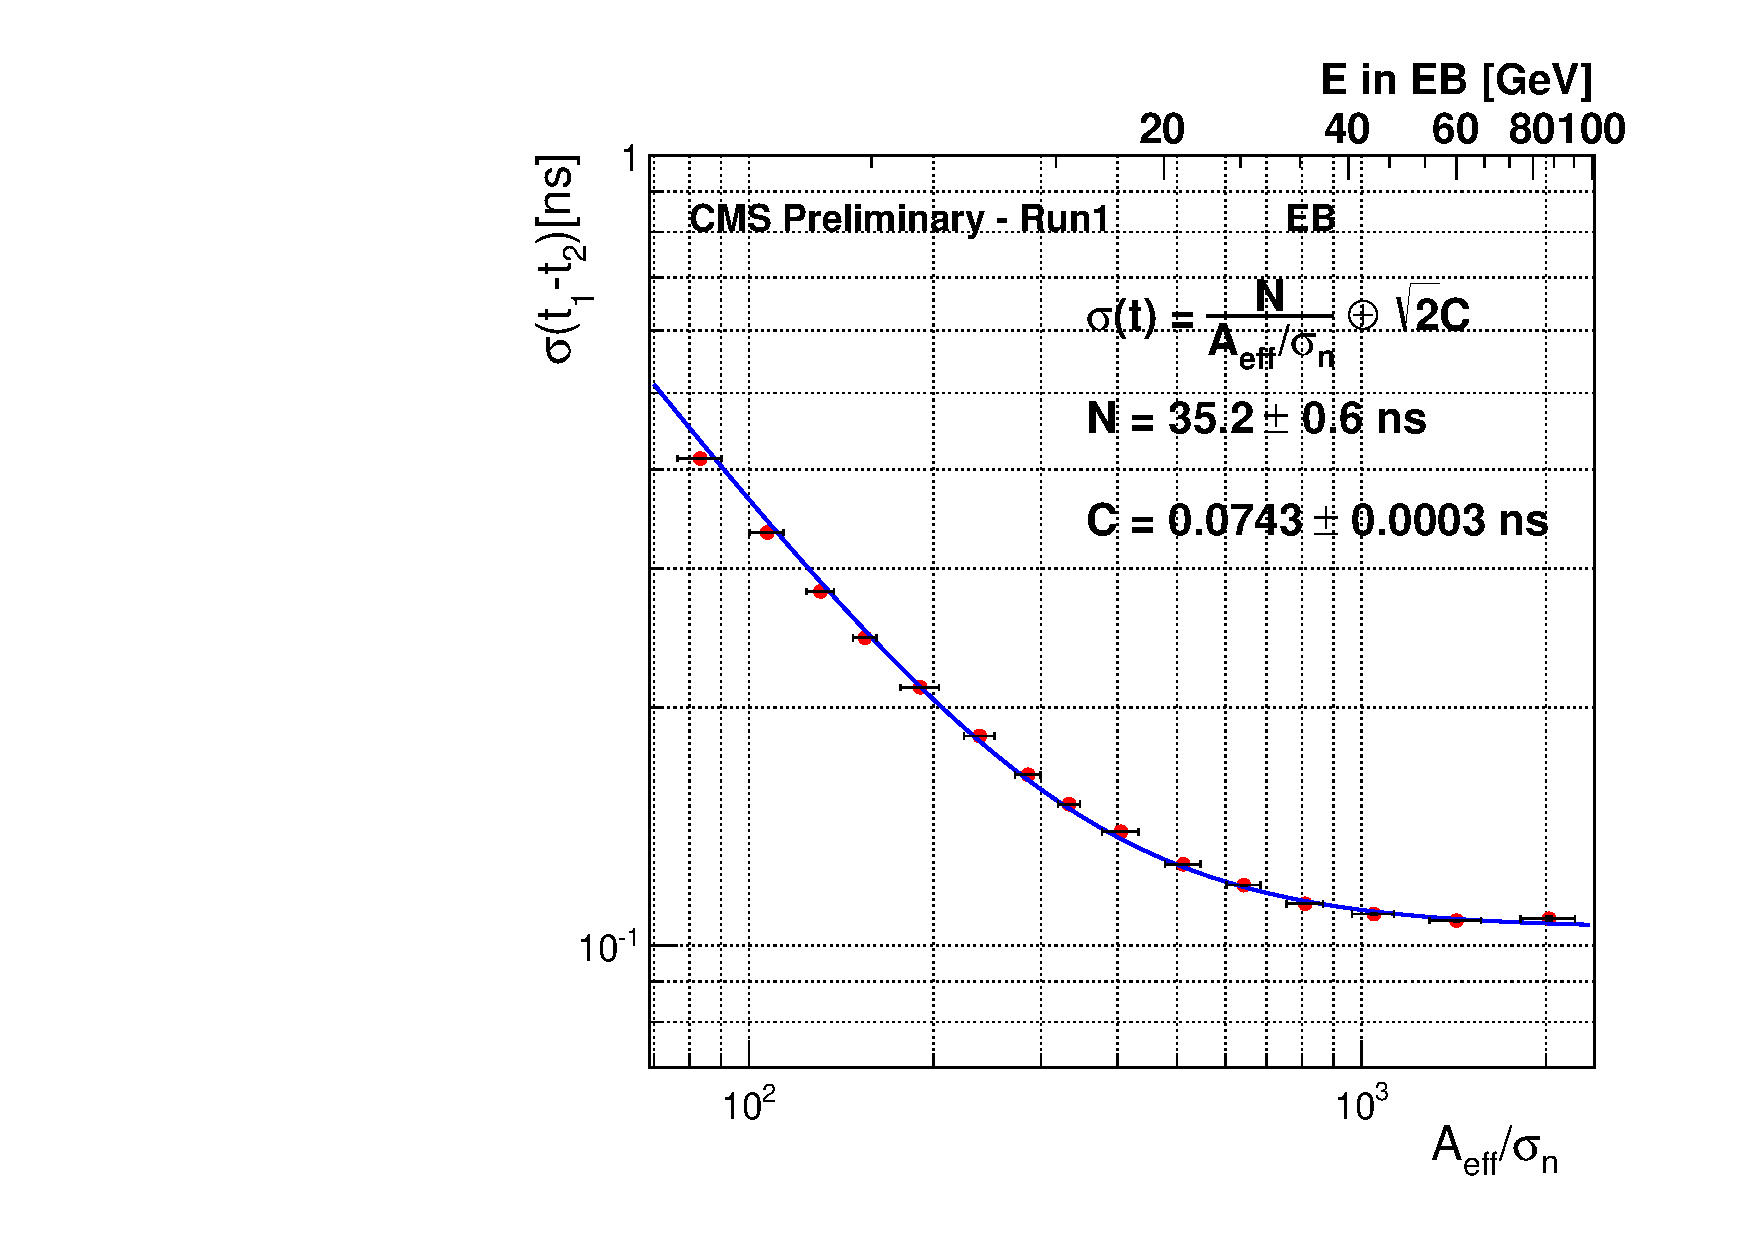
\includegraphics[width=3.0in]{time_resol_neighbors}\label{fig:time_resol_neighbors}}
    \caption{Resolution of time difference between the two electrons from $Z\to ee$ decays, as a function of the effective amplitude $A_{\rm eff}$ defined in the text, normalized to the noise in the ECAL Barrel for Run I data (a). Resolution of time difference between the two most energetic crystals of an ECAL cluster as a function of $A_{\rm eff}$ (b). \label{fig:time_resol}}
  \end{center}
\end{figure}
%


\section{Conclusion}
\label{sec:conclusions}
The electromagnetic calorimeter of CMS has performed optimally during the LHC Run I, and it has been essential in the search for the Higgs boson and in the determination of its properties. The excellent timing performance of the calorimeter has also enabled to extend the CMS reach for physics beyond the Standard Model. The harsh environment of the LHC has required an outstanding effort in the operation, monitoring and calibration, and simulation of the calorimeter. For the forthcoming Run II at $\sqrt{s}=13$ TeV with an increased instantaneous luminosity, an almost doubled number of pile-up interactions and the reduced bunch spacing from 50 ns to 25 ns will make the environment even harsher. 

A new ECAL amplitude reconstruction have been developed and tested, showing that the contribution of the out-of-time pile-up energy can be reduced to a negligible level. 
The consolidated calibration procedures and techniques will be maintained and will serve as the basis for the next data taking period, with a re-optimization of the streams, which has been performed during the shutdown period between Run I and Run II.


% Can use something like this to put references on a page
% by themselves when using endfloat and the captionsoff option.
\ifCLASSOPTIONcaptionsoff
  \newpage
\fi


\begin{thebibliography}{1}

\bibitem{Chatrchyan:2008aa} 
  S.~Chatrchyan {\it et al.}  [CMS Collaboration], ``The CMS experiment at the CERN LHC,'' JINST {\bf 3}, S08004 (2008).

\bibitem{CMS:1997ema} 
  [CMS Collaboration], ``CMS: The electromagnetic calorimeter. Technical design report,''  CERN-LHCC-97-33, CMS-TDR-4.

%\cite{Chatrchyan:2013mxa}
\bibitem{Chatrchyan:2013mxa} 
  S.~Chatrchyan {\it et al.}  [CMS Collaboration], ``Measurement of the properties of a Higgs boson in the four-lepton final state,''
  Phys.\ Rev.\ D {\bf 89}, 092007 (2014)

\bibitem{Khachatryan:2014ira} 
  V.~Khachatryan {\it et al.}  [CMS Collaboration], ``Observation of the diphoton decay of the Higgs boson and measurement of its properties,''  Eur.\ Phys.\ J.\ C {\bf 74}, no. 10, 3076 (2014)

\bibitem{nnls}
J.~Cantarella and M.~Piatek, ``Tsnnls: A solver for large sparse least squares problems with non-negative variables,'' CoRR-cs.MS/0408029 (2004)

\bibitem{Bruneliere:2006ra} 
  P.~Adzic, R.~Alemany-Fernandez, C.~B.~Almeida, N.~M.~Almeida, G.~Anagnostou, M.~G.~Anfreville, I.~Anicin and Z.~Antunovic {\it et al.}, ``Reconstruction of the signal amplitude of the CMS electromagnetic calorimeter,''  Eur.\ Phys.\ J.\ C {\bf 46S1}, 23 (2006).

\bibitem{Chatrchyan:2013dga} 
  S.~Chatrchyan {\it et al.}  [CMS Collaboration], ``Energy Calibration and Resolution of the CMS Electromagnetic Calorimeter in $pp$ Collisions at $\sqrt{s} = 7$ TeV,''   JINST {\bf 8}, P09009 (2013)

\bibitem{Anfreville:2007zz} 
  M.~Anfreville, D.~Bailleux, J.~P.~Bard, A.~Bornheim, C.~Bouchand, E.~Bougamont, M.~Boyer and R.~Chipaux {\it et al.}, ``Laser monitoring system for the CMS lead tungstate crystal calorimeter,''  Nucl.\ Instrum.\ Meth.\ A {\bf 594}, 292 (2008).

\bibitem{CMS:2010eua} 
  [CMS Collaboration], ``Commissioning of the Particle-Flow reconstruction in Minimum-Bias and Jet Events from pp Collisions at 7 TeV,''  CMS-PAS-PFT-10-002.

\bibitem{Chatrchyan:2009aj} 
  S.~Chatrchyan {\it et al.}  [CMS Collaboration], ``Time Reconstruction and Performance of the CMS Electromagnetic Calorimeter,''  JINST {\bf 5}, T03011 (2010)

\bibitem{Gadomski:1992xu} 
  S.~Gadomski, G.~Hall, T.~Hogh, P.~Jalocha, E.~Nygard and P.~Weilhammer, ``The Deconvolution method of fast pulse shaping at hadron colliders,''  Nucl.\ Instrum.\ Meth.\ A {\bf 320}, 217 (1992).

\end{thebibliography}


% that's all folks
\end{document}


